\chapter{S 矩阵的解析性质 (Analytic Properties of the S-matrix)}\label{ch:analytic}

前面几章我们已经在物理动量 $p\geq 0$ 的范围内建立了分波分析的完整框架：
正则解 (regular solution) $\phi_{l,p}(r)$、Jost 解 $\chi^\pm_{l,p}(r)$、
Jost 函数 $f_l(p)$ 以及分波 S 矩阵元 $\Smat_l(p)$。本章的核心目标是把这些函数
解析延拓到复 $p$ 平面上，研究其解析结构 (analyticity, branch cuts, poles)。
S 矩阵的解析性质是散射理论中最重要的结构性质之一：它把束缚态、共振态、阈值
行为等不同物理现象统一在同一个复平面图像中。例如，束缚态对应于 Jost 函数在
正虚轴上的零点 ($p = \rmi\kappa$)，等价地对应分波振幅的极点；准束缚 (virtual)
态出现在负虚轴；共振对应于第二 Riemann 叶上的极点；Levinson 定理则把零能与
高能相移之差直接和束缚态数目联系起来。

本章主要参考 Taylor《Scattering Theory》第 12 章，并按 Xiao 讲义的脉络组织：
(i) 单变量解析函数的若干常用工具；(ii) 正则解关于 $p$ 的整函数性质；
(iii) Jost 函数与 S 矩阵元的解析延拓区域；(iv) 束缚态与 Levinson 定理；
(v) 阈值 $p=0$ 附近的展开 (有效力程展开 / Effective range expansion)。

%======================================================================
\section{单变量解析函数的若干工具}\label{sec:analytic-tools}

我们先列出本章反复使用的复分析工具，作为参考。设 $f(z)$ 是定义在复平面上某
区域 $R$ 内的复函数。

\begin{definition}[解析函数]
$f(z)$ 在区域 $R$ 上\textbf{解析} (analytic, holomorphic)，当且仅当 $f$ 在 $R$
的任意一点都复可微。等价地，$f$ 在 $R$ 内任一点的某个邻域内可以展开为收敛的
Taylor 级数。
\end{definition}

\begin{theorem}[Cauchy 定理与公式]
若 $f$ 在单连通区域 $R$ 内解析，$\gamma\subset R$ 是一条光滑闭曲线，则
\begin{equation}
\oint_\gamma \rmd s\, f(s) = 0,\qquad
f(z) = \frac{1}{2\pi\rmi}\oint_\gamma \frac{f(s)}{s-z}\,\rmd s,
\quad z\text{ 在 }\gamma\text{ 内部}.
\label{eq:cauchy}
\end{equation}
解析函数无穷次可微，且若 $f$ 在 $R$ 中除有限多个极点外解析，则
$\dfrac{1}{2\pi\rmi}\oint \rmd z\, f(z) = \sum_{j} \Res_{z=z_j} f$ (留数定理)。
\end{theorem}

\begin{theorem}[解析延拓的唯一性]
若 $f_1(z)$ 在某条曲线 $\Gamma$ 上有定义，$f_2(z)$ 在包含 $\Gamma$ 的区域 $R$
内解析，且在 $\Gamma$ 上 $f_1=f_2$，则 $f_2$ 是 $f_1$ 由 $\Gamma$ 进入 $R$
的\emph{唯一}解析延拓。
\end{theorem}

\begin{remark}[复共轭与 Schwartz 反射原理]\label{rem:schwartz}
若 $f(z)$ 在 $R$ 内解析，则 $f^*(z)$ 一般\emph{不}在 $R^*=\{z^*:z\in R\}$ 上
解析，但 $[f(z^*)]^*$ 在 $R^*$ 内解析。\textbf{Schwartz 反射原理}：若 $R$ 包含
实轴上的一段，$f$ 在 $R$ 内解析，且当 $z$ 在该段实轴上时 $f(z)\in\R$，则
\begin{equation}
f^*(z) = f(z^*),\qquad z\in R\cup R^*.
\label{eq:schwartz}
\end{equation}
\end{remark}

下面两个定理是把级数展开和参数积分提升为 "解析" 的关键判据。

\begin{theorem}[级数与积分给出的解析函数]\label{thm:series-integral}
\hfill
\begin{enumerate}
\item\emph{(级数求和)}\; 设 $f_n(z)$ 在区域 $R$ 上解析，且级数
$\sum_n f_n(z)$ 在 $R$ 上一致收敛，则 $f(z)=\sum_n f_n(z)$ 在 $R$ 上解析。
\item\emph{(参数积分)}\; 设对每一 $r\in(a,b)\subset\R$，函数 $g(z,r)$ 在 $R$
上解析，且 $g$ 在 $R\times(a,b)$ 上连续，则
$f(z)=\int_a^b\rmd r\,g(z,r)$ 在 $R$ 上解析。
\end{enumerate}
\end{theorem}

\begin{remark}\label{rem:improper}
第二条可以推广到反常积分：当 $a=0$ 时 $g(z,0)$ 发散、或 $b=\infty$、或者
存在某 $r_0$ 处 $g(z,r_0)$ 发散，只要在端点 (与可疑点) 处积分关于 $z$
\emph{一致收敛}，结论仍然成立。这是后面证明 Jost 函数解析性的核心工具。
\end{remark}

%======================================================================
\section{正则解的解析性质}\label{sec:regular-analytic}

考虑约化 Schr\"odinger 径向方程 (取 $2m=1$，势 $U=2mV$)
\begin{equation}
\left[\frac{\rmd^2}{\rmd r^2}-\frac{l(l+1)}{r^2}+p^2-U(r)\right]\psi_l(r)=0.
\label{eq:radial}
\end{equation}
\textbf{正则解} $\phi_{l,p}(r)$ 由 $r\to0$ 处的边界条件
$\phi_{l,p}(r)\sim \hat{j}_l(pr)$ 唯一确定 (其中 $\hat{j}_l(x)=xj_l(x)$，
$\hat{j}_l(x)\to x^{l+1}/(2l+1)!!$ 当 $x\to 0$)。它满足等价的 Volterra
积分方程
\begin{equation}
\phi_{l,p}(r)=\hat{j}_l(pr)+\lambda\int_0^r \rmd r'\,g_{l,p}(r,r')\,U(r')\,\phi_{l,p}(r'),
\label{eq:phi-volterra}
\end{equation}
其中 Green 核为
\begin{equation}
g_{l,p}(r,r')=\frac{1}{p}\bigl[\hat j_l(pr)\hat n_l(pr')-\hat n_l(pr)\hat j_l(pr')\bigr].
\label{eq:greenkernel}
\end{equation}
注意 $\hat j_l, \hat n_l$ 当 $z\to 0$ 分别行为为 $z^{l+1}, z^{-l}$，因此 $g_{l,p}(r,r')$
作为 $p$ 的函数是\emph{整函数} (entire)。

\begin{theorem}[正则解关于 $p$ 是整函数]\label{thm:phi-entire}
对于任意 $p\in\C$ (实或复)，由迭代级数定义的 \eqref{eq:phi-volterra} 解
$\phi_{l,p}(r)$ 关于 $p$ 在整个复平面上解析 (即 $p$ 的整函数)。
\end{theorem}

\begin{proof*}
由 Neumann 迭代展开
\begin{equation}
\phi_{l,p}(r)=\hat j_l(pr)+\sum_{n=1}^\infty \lambda^n\,\phi^{(n)}(r),\qquad
\phi^{(n)}(r)=\frac{1}{p^n}\!\!\int_0^r\!\!\rmd r_n\!\int_0^{r_n}\!\!\rmd r_{n-1}\cdots
\!\int_0^{r_2}\!\!\rmd r_1\,
g_{l,p}(r,r_n)U(r_n)\cdots g_{l,p}(r_2,r_1)U(r_1)\hat j_l(pr_1).
\label{eq:phi-iter}
\end{equation}
对 $l=0$ 分波，$g_{0,p}(r,r')=\sin p(r-r')/p$。利用经典估计
$|\sin z|\leq \beta\,|z|/(1+|z|)\,\rme^{|\Im z|}$ ($\beta$ 是数值常数)，得到
\begin{equation}
|\phi^{(n)}(r)|\leq \beta\,\frac{|pr|}{1+|pr|}\,\rme^{|\Im p|r}\,\frac{\alpha^n}{n!},\qquad
\alpha\equiv\int_0^r\rmd r'\,|U(r')|\,r'.
\label{eq:phi-bound-l0}
\end{equation}
对一般 $l$，类似的估计给出
\begin{equation}
|\phi_{l,p}(r)|\leq \gamma_l\,\Bigl(\frac{|pr|}{1+|pr|}\Bigr)^{l+1}\,\rme^{|\Im p|r},
\label{eq:phi-bound-general}
\end{equation}
其中 $\gamma_l$ 是只依赖于 $l$ 的常数。在 $p$ 的任意有界区域内，$|\phi^{(n)}|$
有共同的可求和上界，故 \eqref{eq:phi-iter} 关于 $p$ 一致收敛；又每一项
$\phi^{(n)}(r)$ 是 $p$ 的整函数 (由定理 \ref{thm:series-integral} 与
注 \ref{rem:improper})，故和也是 $p$ 的整函数。
\end{proof*}

\eqref{eq:phi-bound-general} 同时给出了正则解在大 $|p|$ 下的指数控制：
$|pr|^{l+1}/(1+|pr|)^{l+1}$ 反映了 $\hat j_l(pr)\sim (pr)^{l+1}$ 当 $pr\to 0$
的低能行为，而因子 $\rme^{|\Im p|r}$ 反映了 $\hat j_l(z)\sim\sin(z-l\pi/2)$
当 $|\Im z|\to\infty$ 的高能行为。

\begin{remark}[$p\to-p$ 的对称性]\label{rem:phi-parity}
由 $\hat j_l(-z)=(-1)^{l+1}\hat j_l(z)$，$\hat n_l(-z)=(-1)^l\hat n_l(z)$，可得
$g_{l,-p}(r,r')=g_{l,p}(r,r')$。对积分方程 \eqref{eq:phi-volterra} 两边比较
$p\to -p$ 即得
\begin{equation}
\phi_{l,-p}(r)=(-1)^{l+1}\phi_{l,p}(r).
\label{eq:phi-parity}
\end{equation}
也即 $\phi_{l,p}$ 是 $p$ 的奇 (或偶) 函数，依 $l$ 而定。
\end{remark}

\textbf{两种诠释}\quad 上述结果有两种等价的物理诠释：
\begin{itemize}
\item $\phi_{l,p}(r)$ 是 \eqref{eq:phi-volterra} (复 $p$ 的方程) 的解，关于 $p$
解析，回到物理区域 $p\geq 0$ 时退回物理解；
\item $\phi_{l,p}(r)$ 由物理区域 $p\geq 0$ 上的解析延拓给出复 $p$ 的解。
\end{itemize}
两种观点结合定理 \ref{thm:phi-entire} 给出同一个 $p$ 整函数。

%======================================================================
\section{Jost 函数与分波 S 矩阵元的解析性}\label{sec:jost-analytic}

回顾 Jost 函数的定义：在 $r\to\infty$ 处把正则解写成入射 + 出射球面波的
线性组合
\begin{equation}
\phi_{l,p}(r)\xrightarrow{r\to\infty}
\frac{\rmi}{2}\Bigl[f_l(p)\,\hat h^-_l(pr)-f_l(-p)\,\hat h^+_l(pr)\Bigr],
\label{eq:phi-asymp}
\end{equation}
其中 $\hat h^\pm_l(z)\to (\mp\rmi)^{l+1}\rme^{\pm\rmi z}$ 当 $|z|\to\infty$。
等价地用 Jost 解 $\chi^\pm_{l,p}(r)$ (满足 $\chi^\pm_{l,p}(r)\to\hat h^\pm_l(pr)$)
通过 Wronskian 表达
\begin{equation}
f_l(p)=\frac{1}{p}\,W(\chi^+_{l,p},\phi_{l,p}),\qquad
W(\alpha,\beta)\equiv \alpha\beta'-\alpha'\beta.
\label{eq:fW}
\end{equation}
作为公式更方便的，是积分表达
\begin{equation}
f_l(p)=1+\frac{\lambda}{p}\int_0^\infty \rmd r'\,\hat h^+_l(pr')\,U(r')\,\phi_{l,p}(r').
\label{eq:fl-int-ch11}
\end{equation}
这个式子定义了 $f_l(p)$ 到复 $p$ 平面的解析延拓 (只要积分收敛即可)。

%--------------------------------------------------------------------
\subsection{上半平面的解析性}\label{ssec:upper}

复 $p$ 时，根据 \eqref{eq:phi-bound-general} 与
$|\hat h^+_l(pr)|\leq (\beta|pr|/(1+|pr|))^{-l}\,\rme^{-\Im p\, r}$，
被积函数受控于
\begin{equation}
|\hat h^+_l(pr')\,U(r')\,\phi_{l,p}(r')|
\leq \mathrm{const}\cdot \frac{\beta\,|p|\,r'}{1+|pr'|}\,|U(r')|\,
\rme^{(|\Im p|-\Im p)r'}.
\label{eq:integrand-bound}
\end{equation}
若 $\Im p>0$，则指数因子 $\rme^{(|\Im p|-\Im p)r'}=1$，积分关于 $r'$ 一致收敛
(只要 $r|U(r)|\in L^1$)，由定理 \ref{thm:series-integral} 与
注 \ref{rem:improper}，
\begin{equation}
\boxed{\;f_l(p)\text{ 在上半平面 }\Im p\geq 0\text{ 内解析。}\;}
\label{eq:fl-upper}
\end{equation}

\begin{remark}[势的形态决定下半平面行为]\label{rem:potential-tail}
下半平面的解析性依赖于势的具体长程行为：
\begin{itemize}
\item \textbf{截断势}\,： $r>a$ 时 $U(r)=0$，则 \eqref{eq:fl-int-ch11} 的积分上限
变为 $a$，对所有 $p\in\C$ 收敛，故 $f_l(p)$ 在\emph{整个复平面}上解析
(即 $f_l$ 是整函数)。
\item \textbf{Yukawa 型势} $V\sim \rme^{-\mu r}$\,： \eqref{eq:integrand-bound}
要求 $|\Im p|-\Im p+\mu>0$，即 $\Im p>-\mu/2$，故 $f_l(p)$ 在
$\Im p>-\mu/2$ 解析。
\item 一般 $\rme^{-\mu r}/r$ 型 (Yukawa)\,： $f_l$ 在负虚轴 $p=-\rmi\mu/2,
-\rmi\mu,\ldots$ 处可能有支点 (branch cut)；若 $V\sim\gamma\rme^{-\mu r}$
(非 Yukawa) 则在这些点是\emph{极点}。
\end{itemize}
\end{remark}

%--------------------------------------------------------------------
\subsection{解析势与解析延拓的扩张}\label{ssec:analytic-potential}

若势 $V(r)$ 本身在 $\Re r>0$ 半平面上解析，且对从原点出发的射线 $r=\rho\rme^{\rmi\theta}$
($|\theta|<\pi/2$) 仍有相同的衰减性质，则称之为\textbf{解析势} (analytic
potential)。此时 \eqref{eq:fl-int-ch11} 的 $r$ 积分路径可以变形到复平面上沿射线
$r=\rho\rme^{\rmi\theta}$ 进行：
\begin{equation}
f_l(p)=1+\frac{1}{p}\int_0^{\infty\rme^{\rmi\theta}}\rmd r\,\hat h^+_l(pr)\,U(r)\,\phi_{l,p}(r).
\label{eq:fl-rotated}
\end{equation}
被积函数仍由 \eqref{eq:phi-bound-general} 控制：估计中
$\rme^{|\Im p|r}\to\rme^{|\Im(p\rme^{\rmi\theta})|\rho}$，
$\rme^{-\Im p\,r}\to\rme^{-\Im(p\rme^{\rmi\theta})\rho}$，故关键条件变为
$\Im(p\rme^{\rmi\theta})\geq 0$，即 $p$ 落在以 $-\theta$ 为转角的旋转半平面内。
让 $\theta$ 取遍 $(-\pi/2,\pi/2)$，所有这些半平面的并集是
$\C\setminus(-\rmi\R_+)$ —— 即整个复平面上扣除负虚轴。

\begin{theorem}[解析势的 $f_l$ 解析延拓]
若势 $U(r)$ 在右半平面 $\Re r>0$ 上解析，并对所有从原点出发的射线
$r=\rho\rme^{\rmi\theta}$ 满足前述衰减条件，则 $f_l(p)$ 解析延拓到\emph{除负虚轴
之外}的整个复 $p$ 平面 (Taylor 教材图 12.5)。
\end{theorem}

如果只要求 $V$ 在 $r>a$ 处解析 (而非 $\Re r>0$ 全域)，可选择从 $r=a$ 处弯折
进入复 $r$ 平面的积分路径，结论仍然成立。

\begin{remark}[Yukawa 型势的支割线]
若势同时是解析势 (例如 $V\sim\gamma\rme^{-\mu r}/r$ 是经典 Yukawa)，结合上面两种
情形，$f_l(p)$ 在负虚轴 $p=-\rmi\mu/2,-\rmi\mu,\ldots$ 上有\emph{割线}，
而对纯指数 $V\sim\gamma\rme^{-\mu r}$ 则是\emph{极点}。$\Smat_l(p)$ 在以下
区域内亚纯：
\begin{equation}
-\mu/2<\Im p<\mu/2.
\label{eq:Sl-meromorphic}
\end{equation}
\end{remark}

\begin{remark}[关于下半平面解析性的两点说明]\label{rem:two-remarks}
\begin{enumerate}
\item 对于满足 "上半平面解析" 这种较弱要求的势，要把 $f_l(p)$ 解析延拓到下半
平面需要额外的条件 (例如解析势 / 截断势 / Yukawa)。
\item 物理上 $f_l(p)$ 在下半平面的解析性\emph{并不重要}，下半平面 (尤其负虚轴)
的细节对势的长程行为非常敏感。例如 $\rme^{-\mu r}/r$ 在负虚轴有割线，但若
在 $r>a$ 处截断 ($a$ 很大)，则变成整函数。两种势在物理上不可区分，但解析
结构差别很大。
\end{enumerate}
\end{remark}

%--------------------------------------------------------------------
\subsection{$p\to-p$ 与复共轭对称}\label{ssec:symmetries}

由 $\phi_{l,-p}(r)=(-1)^{l+1}\phi_{l,p}(r)$ 和 $\hat h^+_l(-z)=(-1)^{l+1}\hat h^{+*}_l(z)$
(对实 $z$)，把 $p\to-p$ 代入 \eqref{eq:fl-int-ch11}，对实 $p$ 立刻得到
\begin{equation}
f_l(-p) = [f_l(p)]^*,\qquad p\in\R.
\label{eq:fl-real-conj}
\end{equation}
两边都是 $p$ 的解析函数 (在合适区域内)，由唯一性可解析延拓为
\begin{equation}
\boxed{\;f_l(-p) = [f_l(p^*)]^*,\qquad p\in\C.\;}
\label{eq:fl-schwartz}
\end{equation}
这是 Schwartz 反射原理的直接体现。若 $p$ 在虚轴上 (即 $p^*=-p$)，则
$f_l(-p)=[f_l(-p)]^*$，即 $f_l$ 在虚轴上取实值；$f_l(p)$ 关于虚轴对称两点
互为复共轭。

由 $\Smat_l(p)=f_l(-p)/f_l(p)$ 立得
\begin{equation}
\Smat_l(p)\xrightarrow{p\in\R}\frac{[f_l(p)]^*}{f_l(p)},\qquad
\Smat_l(p)\xrightarrow{p\in\C}\frac{[f_l(p^*)]^*}{f_l(p)}=\frac{f_l(-p)}{f_l(p)}.
\label{eq:Sl-from-fl}
\end{equation}
后两个表达式中，分母关于 $\Im p\geq 0$ 解析，分子关于 $\Im p\leq 0$ 解析。
对于实 $p$ 进而得到\textbf{幺正性恒等式}
\begin{equation}
\Smat_l(p)\,\Smat_l(-p)=\frac{f_l(-p)}{f_l(p)}\cdot\frac{f_l(p)}{f_l(-p)}=1,\qquad
|\Smat_l(p)|^2 = 1.
\label{eq:unitarity}
\end{equation}

%======================================================================
\section{Riemann 面上的 S 矩阵：$E$ 平面图像}\label{sec:riemann}

物理能量与动量的关系是 $E=p^2/(2m)$ (取 $2m=1$ 时 $E=p^2$)。从 $p$ 平面到
$E$ 平面的映射是 2 对 1 的：$\pm p$ 对应同一个 $E$。因此在 $E$ 平面上
$\Smat_l$ 一般是 \emph{Riemann 双叶面} 上的函数：

\begin{itemize}
\item \textbf{物理叶 (physical sheet)}\,：对应 $p$ 平面的上半 $\Im p>0$，
覆盖 $E$ 平面剪开沿正实轴 ($E\geq 0$, 散射阈值之上) 的区域；正能 $E>0$
对应 $p\in\R_+$。
\item \textbf{第二叶 (second / unphysical sheet)}\,：对应 $\Im p<0$，
通过把 $E$ 平面割线上下唇粘合得到。
\end{itemize}

物理叶上 (上半 $p$ 平面)，$\Smat_l$ 在束缚态对应的正虚轴点
$p=\rmi\kappa_n$ 处有极点 (实际上是 $f_l(p)$ 的零点)；负实能 $E_n=-\kappa_n^2/(2m)<0$。
第二叶上 (下半 $p$ 平面) 的极点 $p=p_R-\rmi\Gamma/2$ 对应共振，$E_R=p_R^2-\rmi p_R\Gamma$
位于实轴下方。\emph{虚态}\, (virtual / antibound state) 是负虚轴上的零点
$p=-\rmi\kappa$，对应负 $E$，但在第二叶上而非物理叶。

%======================================================================
\section{束缚态与 Levinson 定理}\label{sec:bound-states}

%--------------------------------------------------------------------
\subsection{束缚态对应 Jost 函数的零点}\label{ssec:bound-zeros}

回到渐近形式 \eqref{eq:phi-asymp}。当 $\Im p>0$ 时，$\hat h^+_l(pr)\to0$ 而
$\hat h^-_l(pr)\to\infty$。设在某 $\bar p$ ($\Im\bar p>0$) 处
$f_l(\bar p)=0$，则 \eqref{eq:phi-asymp} 中 "上升" 项消失，剩
\begin{equation}
\phi_{l,\bar p}(r)\xrightarrow{r\to\infty}
-\frac{\rmi}{2}f_l(-\bar p)\,\hat h^+_l(\bar p r)
\sim \rme^{\rmi(\bar p r-l\pi/2)},
\end{equation}
当 $\Im\bar p>0$ 时这是\emph{指数衰减}的，配合 $\phi_{l,\bar p}(0)=0$，
$\phi_{l,\bar p}$ 是平方可积的——恰是 Schr\"odinger 方程的束缚态波函数。

由于 $\Hmat$ 是 Hermitian 算符，束缚态本征值 $E=p^2/(2m)$ 必为实，故
$\bar p$ 必为\emph{纯虚数}：$\bar p=\rmi\kappa$ ($\kappa>0$)，$E=-\kappa^2/(2m)$。

\begin{theorem}[束缚态 $\Leftrightarrow$ Jost 函数零点]\label{thm:bound-zero}
对满足前述条件的中心势 $V(r)$，每一个角动量 $l$ 子空间内的束缚态 (本征值
$E_n=-\kappa_n^2/(2m)<0$) 与 Jost 函数 $f_l(p)$ 在正虚轴上的一阶零点
$p=\rmi\kappa_n$ 一一对应；等价地与分波 S 矩阵元 $\Smat_l(p)=f_l(-p)/f_l(p)$
在正虚轴上的一阶极点一一对应。
\end{theorem}

\begin{proof*}\!(简要)
设 $f_l(\bar p)=0$，$\Im\bar p>0$。由 Wronskian 表达 \eqref{eq:fW}，
$W(\chi^+_{l,\bar p},\phi_{l,\bar p})=0$，故 $\chi^+_{l,\bar p}$ 与
$\phi_{l,\bar p}$ 线性相关：$\phi_{l,\bar p}(r)=\lambda\,\chi^+_{l,\bar p}(r)$。
$\chi^+_{l,\bar p}(r)\to\hat h^+_l(\bar p r)$ 指数衰减，故 $\phi_{l,\bar p}$
平方可积且满足 Schr\"odinger 方程，$E=\bar p^2/(2m)$ 是束缚态能量。反过来
若有束缚态，则同样的 $\phi_{l,\bar p}\propto\chi^+_{l,\bar p}$ 关系成立，
推出 $f_l(\bar p)=0$。

\textbf{零点为单阶}：考虑 $\rmd f_l/\rmd p$。利用 \eqref{eq:fl-int-ch11} 的等价积分
表达 (经辐向方程的 Wronskian 操作可化为)
\begin{equation}
\frac{\rmd f_l}{\rmd p}(\bar p)=\int_0^\infty \rmd r\,\chi^+_{l,\bar p}(r)\,\phi_{l,\bar p}(r)
=\lambda\int_0^\infty \rmd r\,[\chi^+_{l,\bar p}(r)]^2\neq 0,
\end{equation}
因为束缚态波函数本身归一化非零。详见 Taylor 习题 12.3。
\end{proof*}

\begin{remark}[分波振幅的留数]
分波振幅 $f_l^{\text{amp}}(p)=[\Smat_l(p)-1]/(2\rmi p)$ 在 $\bar p=\rmi\kappa_n$
处是一阶极点，留数为
\begin{equation}
\Res_{p=\rmi\kappa_n}\Smat_l(p) = \frac{f_l(-\rmi\kappa_n)}{(\rmd f_l/\rmd p)|_{\rmi\kappa_n}}.
\end{equation}
对 $E$ 平面：分波振幅在 $E_n=-\kappa_n^2/(2m)$ 处的留数为
$\Gamma_n=(-1)^{l+1}\gamma_n^2/(2m)$，其中 $\gamma_n$ 是归一化束缚态径向波函数
在 $r\to\infty$ 处的渐近形式 $\eta(r)\to\gamma_n\rme^{-\kappa_n r}$ 中的常数
(见 Taylor 习题 12.3)。
\end{remark}

%--------------------------------------------------------------------
\subsection{Levinson 定理}\label{ssec:levinson}

\begin{theorem}[Jost 函数关于 $p$ 的两个性质]\label{thm:fl-properties}
\hfill
\begin{enumerate}
\item $f_l(p)$ 在实轴上 (除可能 $p=0$ 外) 不能取零值；
\item 当 $|p|\to\infty$ 且 $\Im p\geq 0$ 时，$f_l(p)\to 1$，更精确地
\begin{equation}
f_l(p)-1 = O(|p|^{-\eta}),\qquad |p|\to\infty,\ \Im p\geq 0,
\label{eq:fl-large}
\end{equation}
均匀地对某 $\eta>0$ 成立。
\end{enumerate}
\end{theorem}

\begin{proof*}
1) 若实 $p\neq 0$ 满足 $f_l(p)=0$，则也有 $f_l^*(p)=f_l(-p)=0$。
渐近式 \eqref{eq:phi-asymp} 的两个 "Hankel" 项同时消失，结合
$r\to 0$ 处 $\phi_{l,p}(r)\to (pr)^{l+1}/(2l+1)!!\neq 0$ (除非 $p=0$)，
得 $\phi_{l,p}\equiv 0$，矛盾。

2) 由 \eqref{eq:fl-int-ch11} 估计被积函数即得；详见上一章关于 Jost 函数大 $p$
渐近的讨论的复 $p$ 推广。
\end{proof*}

\begin{corollary}[束缚态有限性]\label{cor:bound-finite}
对固定的 $l$，$f_l(p)$ 在上半平面 $\Im p>0$ 中只有\emph{有限个}零点，即只有
有限个束缚态。 ($p=0$ 处需特殊考虑，见 \S\ref{sec:threshold}。)
\end{corollary}

\begin{proof*}
由性质 2，存在 $p_0>0$ 使得 $|p|>p_0$ 时 $f_l(p)\neq 0$；上半平面内 $|p|\leq p_0$
是有界闭区域，解析函数在有界闭区域上不能有无穷多孤立零点。
\end{proof*}

\begin{theorem}[Levinson 定理]\label{thm:levinson}
对球对称势 $V(r)$ (满足前面的衰减条件)，分波 $l$ 的相移 $\delta_l(p)$ 满足
\begin{equation}
\boxed{\;\delta_l(0)-\delta_l(\infty) = n_l\,\pi\;}
\label{eq:levinson}
\end{equation}
其中 $n_l$ 是分波 $l$ 中的束缚态个数。例外情形：当 $l=0$ 且 $f_0(0)=0$ 时
("零能 s 波束缚态")，则
\begin{equation}
\delta_0(0)-\delta_0(\infty) = (n_0+\tfrac{1}{2})\pi.
\label{eq:levinson-exc}
\end{equation}
\end{theorem}

\begin{proof*}\!(主要思想，$f_l(0)\neq 0$ 情形)
考察上半平面的辐角原理积分
\begin{equation}
I=\oint \rmd\ln f_l(p) = \oint \rmd p\,\frac{f_l'(p)}{f_l(p)} = 2\pi\rmi\,n_l,
\label{eq:argprinciple}
\end{equation}
其中环路取 "大半圆"：实轴 $p\in[-R,R]$ 加 $|p|=R$ 的上半圆 (取 $R\to\infty$)。

(i) 实轴上 ($p>0$)，由 $|f_l|^2$ 在分波幺正性下与相移的关系
$f_l(p)=|f_l(p)|\rme^{-\rmi\delta_l(p)}$，并利用 $f_l(-p)=f_l^*(p)$ 反演到 $p<0$
段。综合两段实轴贡献：
\begin{equation}
I_{\text{real}}=\int_{-\infty}^\infty\rmd\ln f_l(p) = -2\rmi\int_0^\infty\rmd\delta_l(p)
=-2\rmi[\delta_l(\infty)-\delta_l(0)].
\end{equation}
(ii) 大半圆 $|p|=R\to\infty$ 上，$f_l\to 1$，故 $\rmd\ln f_l\to 0$，圆上贡献
为零。

合起来 $-2\rmi[\delta_l(\infty)-\delta_l(0)]=2\pi\rmi n_l$，即
$\delta_l(0)-\delta_l(\infty)=n_l\pi$。
\end{proof*}

\begin{remark}[$f_l(0)=0$ 例外情形]
若 $l=0$ 且 $f_0(0)=0$ (即在阈值 $p=0$ 处恰有一个 "零能束缚态"，物理上对应散射
长度发散)，则环路在 $p=0$ 处需绕一个小半圆 $\Gamma_\epsilon$。该小半圆贡献
$-\pi\rmi$ ($l=0$ 时 $f_0(p)\sim\rmi\gamma p$，$\rmd\ln f_0/\rmd p\sim 1/p$)
或 $-2\pi\rmi$ ($l>0$ 时 $f_l(p)\sim\beta p^2$，零点为二阶根)。详细计算见
\S\ref{ssec:threshold-zero}。
\end{remark}

%======================================================================
\section{阈值 $p=0$ 附近的行为}\label{sec:threshold}

阈值是物理动量与解析延拓的交界，散射截面的低能行为由 $p=0$ 处
$f_l(p),\Smat_l(p)$ 的展开主导。

%--------------------------------------------------------------------
\subsection{$f_l(0)\neq 0$ 时的展开}\label{ssec:threshold-nonzero}

分波振幅可写为
\begin{equation}
f_l^{\text{amp}}(p)=\frac{\Smat_l(p)-1}{2\rmi p}
=\frac{f_l(-p)-f_l(p)}{2\rmi p\,f_l(p)}
=-\frac{1}{p^2 f_l(p)}\int_0^\infty\rmd r\,\hat j_l(pr)\,U(r)\,\phi_{l,p}(r).
\label{eq:amp-int}
\end{equation}
利用 $|\hat j_l(pr)|,|\phi_{l,p}(r)|\leq \mathrm{const}\cdot[pr/(1+pr)]^{l+1}$，
若 $f_l(0)\neq 0$，则
\begin{equation}
|f_l^{\text{amp}}(p)|\leq \frac{\mathrm{const}}{|f_l(0)|}\,\frac{1}{|p|^2}
\int_0^\infty \rmd r\,|U(r)|\,\Bigl(\frac{|p|r}{1+|p|r}\Bigr)^{2l+2}.
\label{eq:amp-bound}
\end{equation}
对指数压低 (Yukawa 型) 的势，分母 $1+pr\to 1$ ($p\to 0$ 与 $r$ 实际范围有限
共同保证)，故 $f_l^{\text{amp}}(p)=O(p^{2l})$。等价的 Taylor 展开
\begin{equation}
\boxed{\;f_l^{\text{amp}}(p)=-a_l\,p^{2l}+b_l\,p^{2l+1}+\cdots,\qquad p\to 0\;}
\label{eq:scattering-length}
\end{equation}
其中 $a_l$ 是有限常数 (可能为零)，$l=0$ 时即为\textbf{散射长度} (scattering length)。

\begin{remark}[长程势的破坏]
当 $r\to\infty$ 时 $V(r)=O(1/r^\nu)$ ($\nu>0$，幂律 tail) 而非指数衰减时，
\eqref{eq:amp-bound} 中分母 $1+pr$ 不能直接置 $1$，需要更细致的分析：
\begin{itemize}
\item $l<(\nu-3)/2$ 时积分仍收敛，$f_l^{\text{amp}}=O(p^{2l})$；
\item $l>(\nu-3)/2$ 时积分需保留 $1+pr$ 因子，结果是 $f_l^{\text{amp}}=O(p^{\nu-3})$。
\end{itemize}
此时 $p=0$ 处的解析行为未知，不一定能展开为整次幂。例如 $1/r^4$ tail 给出
$p\cot\delta_0(p)=-1/a_0+bp+cp^2\ln p+O(p^2)$ (含对数项)。
\end{remark}

%--------------------------------------------------------------------
\subsection{有效力程展开 (Effective range expansion)}\label{ssec:effective-range}

对 $f_l(0)\neq 0$ 的情形，引入分波振幅的 \emph{K 矩阵参数化}
\begin{equation}
\Smat_l(p)=\frac{1+\rmi k_l(p)}{1-\rmi k_l(p)},\qquad
k_l(p)=\rmi\,\frac{1-\Smat_l(p)}{1+\Smat_l(p)}=\tan\delta_l(p).
\label{eq:K-matrix}
\end{equation}
对实 $p>0$，$k_l(p)$ 实，$\Smat_l$ 自动幺正。除 $\Smat_l=-1$ (此即
$\delta_l=\pi/2$，相对应 K 矩阵奇点) 外，$k_l$ 在 $\Smat_l$ 解析的点处解析，
\emph{特别地在 $p=0$ 处解析} (假设 $f_l(0)\neq 0$)。

由 $\Smat_l(-p)=1/\Smat_l(p)$ 推出 $k_l(-p)=-k_l(p)$，是 $p$ 的奇函数。结合
低能行为 $\delta_l(p)\to a_l p^{2l+1}$ 给出
\begin{equation}
k_l(p)\xrightarrow{p\to 0} -a_l\,p^{2l+1}.
\label{eq:kl-low}
\end{equation}
故 $k_l/p^{2l+1}$ 是 $p^2$ 的偶函数且在原点解析，可展开为
\begin{equation}
\boxed{\;\frac{p^{2l+1}}{k_l(p)} = p^{2l+1}\cot\delta_l(p)
= -\frac{1}{a_l}+\frac{r_l}{2}\,p^2+O(p^4)\;}
\label{eq:eff-range-ch11}
\end{equation}
这就是著名的\textbf{有效力程展开}。其中：
\begin{itemize}
\item $a_l$\,：分波 $l$ 的散射长度；
\item $r_l$\,：分波 $l$ 的有效力程 (effective range)；对 $l=0$，$r_0$ 物理近似
等于势的有效范围。
\end{itemize}
仅取前两项的近似称为\textbf{有效力程近似} (effective range approximation)。
对 $n$-$p$ 散射，能量低于 $10\,\mathrm{MeV}$ 时该近似精度很高。

\begin{remark}[$1/r^\nu$ tail 破坏 $p^2$ 展开]
对长程 $1/r^\nu$ 型势，$\Smat_l(p)$ 在 $p=0$ 一般含有支点 (例如
$1/r^4$ tail 给出 $p\cot\delta_0=-1/a_0+bp+cp^2\ln p+O(p^2)$)，无法做关于
$p^2$ 的整次幂 effective range expansion。
\end{remark}

%--------------------------------------------------------------------
\subsection{阈值零点 $f_l(0)=0$}\label{ssec:threshold-zero}

考虑特殊情形 $f_l(0)=0$。$p=0$ 时径向方程退化为
\begin{equation}
\Bigl[\frac{\rmd^2}{\rmd r^2}-\frac{l(l+1)}{r^2}-U(r)\Bigr]y(r)=0,
\end{equation}
$r\to 0,\infty$ 由 $l(l+1)/r^2$ 项主导：
\begin{itemize}
\item $r\to 0$\,： $y(r)\sim r^{l+1}$；
\item $r\to\infty$\,： 自由解 $y\sim r^{l+1}$ 与 $y\sim 1/r^l$，物理选择
$1/r^l$。
\item 对 $l=0$， $r\to\infty$，$y\sim 1/r^0=$ 常数，\emph{不可归一化}，故
\emph{不是}束缚态。
\item 对 $l>0$， $y\sim 1/r^l$ 平方可积 (在 $r\to\infty$ 端)，\emph{可以}是
束缚态 (零能束缚态)。
\end{itemize}
能否两端同时满足，依赖势的细节，只对特殊解才存在。

\textbf{$f_l(p)$ 在 $p=0$ 趋零的方式}\quad 假设势指数衰减，可以在 \eqref{eq:fl-int-ch11}
内展开 $\hat h^+_l(pr)=\hat n_l(pr)+\rmi\hat j_l(pr)$：
\begin{align}
f_l(p)&=1+\frac{1}{p}\int_0^\infty\rmd r\,\hat n_l(pr)\,U(r)\,\phi_{l,p}(r)
+\frac{\rmi}{p}\int_0^\infty\rmd r\,\hat j_l(pr)\,U(r)\,\phi_{l,p}(r)\\
&\xrightarrow{p\to 0} 1+[\alpha_l+\beta_l p^2+O(p^4)]+\rmi[\gamma_l p^{2l+1}+O(p^{2l+3})].
\label{eq:fl-zero-expand}
\end{align}
注意 $\hat j_l, \hat n_l, \phi_{l,p}$ 是实的 (对实 $p$)，故 $\alpha_l,\beta_l,\gamma_l$
都是实数。利用 $f_l(0)=0$ 得 $\alpha_l=-1$，故
\begin{equation}
f_l(p)=[\beta_l p^2+O(p^4)]+\rmi[\gamma_l p^{2l+1}+O(p^{2l+3})].
\end{equation}
比较实部虚部最低阶：
\begin{equation}
l=0\,:\ f_0(p)=\rmi\gamma_0 p+O(p^2)\ (\text{单阶根}),\qquad
l>0\,:\ f_l(p)=\beta_l p^2+O(p^3\text{ 或 }p^4)\ (\text{二阶根}).
\label{eq:fl-zero-orders}
\end{equation}
即 $l=0$ 时 $p=0$ 是 $f_0$ 的简单零点；$l\geq 1$ 时是二阶零点。

\textbf{Levinson 定理在 $f_l(0)=0$ 时的修正}\quad 把
\eqref{eq:argprinciple} 的环路修改为绕 $p=0$ 的小半圆 $\Gamma_\epsilon$：
\begin{equation}
I=2\rmi[\delta_l(0)-\delta_l(\infty)]+\lim_{\epsilon\to 0}\int_{\Gamma_\epsilon}\rmd p\,
\frac{f_l'(p)}{f_l(p)}.
\end{equation}
小半圆贡献：$l=0$ 时 $f_0'/f_0\sim 1/p$，半圆给 $-\pi\rmi$；$l>0$ 时
$f_l'/f_l\sim 2/p$，给 $-2\pi\rmi$。结合 $I=2\pi\rmi n_l(\Im p>0)$
(其中 $l=0$ 的 $p=0$ 不算束缚态，$l>0$ 的算)，得
\begin{equation}
\delta_l(0)-\delta_l(\infty)=
\begin{cases}
(n_0+\tfrac{1}{2})\pi, & l=0,\\
n_l\,\pi, & l>0.
\end{cases}
\label{eq:levinson-corrected}
\end{equation}
对 $l>0$，零能 $1/r^l$ 解\emph{可}归一化故被算在束缚态总数 $n_l$ 内；对 $l=0$，
零能解不可归一化，于是出现额外的 $\pi/2$。

\textbf{阈值附近分波振幅的行为}\quad 由
$f_l^{\text{amp}}(p)=-1/(p^2 f_l(p))\cdot\int_0^\infty\rmd r\,\hat j_l(pr)U(r)\phi_{l,p}(r)$
\begin{itemize}
\item $f_l(0)\neq 0$\,：$f_l^{\text{amp}}=-a_l p^{2l}+O(p^{2l+1})$，常规阈值。
\item $l=0$, $f_0(0)=0$\,：$f_0\sim \rmi\gamma_0 p$，
$\hat j_0(pr)\sim p$，$\phi_{0,p}\sim p$，所以
\begin{equation}
f_0^{\text{amp}}(p)=\frac{\rmi a_0}{p}+O(1),\qquad a_0\in\R.
\end{equation}
对应 $\delta_0(0)=\pi/2\pmod\pi$, $\sin\delta_0\to\rmi$ 形式上发散，截面
$\sigma_0=4\pi|f_0^{\text{amp}}|^2\to\infty$ —— 即 \emph{零能共振}
(zero-energy resonance / scattering length divergence)。
\item $l>0$, $f_l(0)=0$\,：$f_l\sim\beta_l p^2$，相比 $f_l\neq 0$ 情形分母多了
$p^2$，所以
\begin{equation}
f_l^{\text{amp}}(p)=a_l p^{2l-2}+O(p^{2l-1}),
\end{equation}
低能幂次比 \eqref{eq:scattering-length} 减少两次。
\end{itemize}

%======================================================================
\section{Wronskian 与几个有用的等式}\label{sec:wronskian}

为完整起见，列出本章使用的 Wronskian 性质。给定两函数 $\alpha(r),\beta(r)$，
\begin{equation}
W(\alpha,\beta)=\alpha\beta'-\alpha'\beta=\det\begin{pmatrix}\alpha&\beta\\
\alpha'&\beta'\end{pmatrix}.
\end{equation}
若 $\alpha,\beta$ 线性相关则 $W\equiv 0$。若 $\alpha,\beta$ 都满足同一径向方程
\eqref{eq:radial}，则 $W'=0$，即 $W$ 与 $r$ 无关。常用值：
\begin{equation}
W(\hat j_l(pr),\hat n_l(pr))=-p,\qquad
W(\chi^+_{l,p},\chi^-_{l,p})=-2\rmi p.
\end{equation}
由此 \eqref{eq:fW} 给出 $f_l(p)=W(\chi^+_{l,p},\phi_{l,p})/p$。
若 $f_l(\bar p)=0$ ($\Im\bar p>0$)，则 $W(\chi^+_{l,\bar p},\phi_{l,\bar p})=0$，
$\phi_{l,\bar p}\propto\chi^+_{l,\bar p}$，二者均指数衰减，平方可积，给出束缚态。

%======================================================================
\section{Jost 解 $\chi^\pm_{l,p}$ 的解析性}\label{sec:jost-solutions}

定义径向方程关于纯出射 / 入射的 Jost 解
\begin{equation}
\chi^\pm_{l,p}(r)\xrightarrow{r\to\infty}\hat h^\pm_l(pr).
\end{equation}
一般来说 $\chi^\pm_{l,p}(r)$ 在 $r=0$ 处不为零，并不正比于正则解
$\phi_{l,p}$。它们满足 Volterra 型积分方程 (积分上限是无穷)
\begin{equation}
\chi^\pm_{l,p}(r)=\hat h^\pm_l(pr)-\int_r^\infty\rmd r'\,g_{l,p}(r,r')\,U(r')\,\chi^\pm_{l,p}(r'),
\label{eq:chi-volterra}
\end{equation}
$g_{l,p}$ 与正则解的 Green 核相同。可由迭代求解：
\begin{itemize}
\item $\chi^+_{l,p}(r)$ 在 $\Im p\geq 0$ 存在，是径向方程的解，关于 $r$ 连续，
关于 $p$ 在 $\Im p>0$ 解析；
\item $\chi^-_{l,p}(r)$ 在 $\Im p\leq 0$ 存在，关于 $p$ 在 $\Im p<0$ 解析。
\end{itemize}
对实 $p$，$\phi_{l,p}$ 与 $\chi^\pm_{l,p}$ 由 \eqref{eq:phi-asymp} 联系：
\begin{equation}
\phi_{l,p}(r)=\frac{\rmi}{2}\bigl[f_l(p)\,\chi^-_{l,p}(r)-f_l(-p)\,\chi^+_{l,p}(r)\bigr],\qquad p\in\R.
\end{equation}

%======================================================================
\section{小结：解析结构图像}\label{sec:summary}

我们已建立了如下统一图像：

\begin{itemize}
\item 正则解 $\phi_{l,p}(r)$ 是 $p$ 的整函数；
\item Jost 函数 $f_l(p)$ 在上半 $p$ 平面 $\Im p\geq 0$ 解析；下半平面解析性
依赖势的长程行为：截断势给出 $f_l$ 整函数，Yukawa 给出极点 / 割线在
$p=-\rmi\mu/2,-\rmi\mu,\ldots$；
\item 实轴对称：$f_l(-p)=[f_l(p^*)]^*$；
\item $\Smat_l(p)=f_l(-p)/f_l(p)$ 在适当区域内是亚纯的；满足
$\Smat_l(p)\Smat_l(-p)=1$，$|\Smat_l(p)|=1$ ($p\in\R$)，$\Smat_l(-p^*)=\Smat_l(p)^*$；
\item \textbf{束缚态} $\Leftrightarrow$ $f_l$ 在正虚轴 $p=\rmi\kappa_n$ 的零点
$\Leftrightarrow$ $\Smat_l$ 的极点；束缚态有限多 (定理 \ref{cor:bound-finite})；
\item \textbf{虚态} $\Leftrightarrow$ $f_l$ 在负虚轴的零点 (在 $E$ 平面第二叶
上的负实能极点)；
\item \textbf{共振} $\Leftrightarrow$ $f_l$ 在下半 $p$ 平面 (第二叶) 的零点，
$\Smat_l$ 的极点 $p=p_R-\rmi\Gamma/2$；
\item \textbf{Levinson 定理}\,： $\delta_l(0)-\delta_l(\infty)=n_l\pi$ (例外
情形 $l=0,f_0(0)=0$ 时为 $(n_0+1/2)\pi$)；
\item \textbf{阈值行为}\,：常规情形 $f_l^{\text{amp}}(p)=-a_l p^{2l}+O(p^{2l+1})$；
有效力程展开
$p^{2l+1}\cot\delta_l(p)=-1/a_l+r_l p^2/2+O(p^4)$ 适用于指数衰减势。
\end{itemize}

下一章 \ref{ch:resonance} 我们将进一步讨论共振 (resonance) 作为第二叶上极点
的物理诠释、Breit--Wigner 公式以及共振对截面与时延的影响。

%======================================================================
\section{逆散射问题：Marchenko 与 Gelfand--Levitan 方程}\label{sec:anlyt-inverse}

到目前为止我们讨论的是\emph{正问题 (direct problem)}：给定势 $V(r)$, 推导 Jost 函数 $f_l(p)$、$\Smat_l$、束缚态等. \textbf{逆问题 (inverse problem)} 反过来问: 给定实轴上 $\Smat_l(p)$ (相移 $\delta_l$) + 束缚态能量 $\{-\kappa_n^2/(2m)\}_{n=1}^{N}$ + 束缚态归一化常数 $\{c_n\}$, 能否\emph{唯一}重构势 $V(r)$？

这是 Marchenko (1955)、Gelfand--Levitan (1951)、Faddeev (1959) 等人发展起来的经典 \textbf{逆散射理论 (Inverse Scattering Theory, IST)}; 它不仅是数学物理的优美课题, 也是\emph{可积系统}量子方法的基础 (KdV、sine-Gordon 等的逆散射解法). 本节给出最简版本 ($l=0$、短程势) 的 Marchenko 方程及其使用方法.

\subsection{逆问题的提法}\label{ssec:anlyt-inverse-setup}

\begin{definition}[散射数据]\label{def:inv-data}
  对中心势 $V(r)$ 的 $s$ 波散射, \emph{散射数据集 (scattering data)}
  \begin{equation}
    \mathcal S=\bigl\{\,\Smat_0(p)\ \text{for}\ p\in\R_+,\ \{\kappa_n,c_n\}_{n=1}^{N}\bigr\}
    \label{eq:inv-data}
  \end{equation}
  包含:
  \begin{enumerate}
    \item 正实轴 $p>0$ 上的 $\Smat_0(p)=\rme^{2\rmi\delta_0(p)}$ (等价: 相移 $\delta_0(p)$);
    \item 束缚态参数: $N$ 个 $s$ 波束缚态, 衰减率 $\kappa_n>0$ 对应能量 $E_n=-\kappa_n^2/(2m)$;
    \item 束缚态归一化常数 (\emph{ANC, asymptotic normalization constants}):
    \begin{equation}
      c_n^2=\biggl[\int_0^\infty\rmd r\,|\phi_n(r)|^2\biggr]^{-1}
      =\biggl[\rmi\,\dot f_0(\rmi\kappa_n)\,f_0(-\rmi\kappa_n)\biggr]^{-1},
      \label{eq:inv-cn}
    \end{equation}
    即把束缚态约化波函数渐近规范化为 $\phi_n(r)\sim c_n\rme^{-\kappa_n r}$ 时所需的常数. $\dot f_0$ 是 $f_0$ 关于 $p$ 的导数.
  \end{enumerate}
\end{definition}

逆问题问: 给定 $\mathcal S$, 能否找到 $V(r)$ 使其 $s$ 波散射数据恰好是 $\mathcal S$? 是否唯一?

\begin{remark}[为什么需要 $c_n$ 而非只 $\kappa_n$]
  仅给 $\delta_0(p)$ 与 $\{\kappa_n\}$ 不足以唯一确定 $V$. 例如, \emph{Bargmann 反射势族}给出一类势 $V_\lambda(r)$, 它们有完全相同的 $\delta_0(p)$ 与束缚态能量, 但 ANC $c_n$ 不同——对应物理上"束缚态在外部空间的强度"不同. 这就是\textbf{相位等价势 (phase-equivalent potentials)}的来源, 详见 Chadan--Sabatier 第 4 章.
\end{remark}

\subsection{由散射数据构造的核函数 $F$}\label{ssec:anlyt-Fkernel}

定义\emph{反射系数} (对 $s$ 波约定):
\begin{equation}
  R(p)\equiv\frac{\Smat_0(p)-1}{2}\,(\text{或等价的归一化}),\qquad p\in\R.
  \label{eq:inv-R}
\end{equation}
不同文献约定有差别, 通常取 $R(p)=\bigl[1-\Smat_0(p)\bigr]/2$ 或 $-\rmi\bigl[\Smat_0(p)-1\bigr]/(2p)$ 等. 这里采用 Marchenko 原始约定
\begin{equation}
  R(p)=\frac{1-\Smat_0(p)}{2\pi},
\end{equation}
将之后的 Fourier 因子分配得最简洁.

\begin{definition}[Marchenko 核 $F(r)$]\label{def:inv-Fkernel}
  由散射数据 $\mathcal S$ 构造
  \begin{empheq}[box=\fbox]{equation}
    F(x)\equiv\sum_{n=1}^{N}c_n^2\,\rme^{-\kappa_n x}+\int_{-\infty}^{\infty}\rmd p\,R(p)\,\rme^{\rmi p x},\qquad x>0.
    \label{eq:inv-Fkernel}
  \end{empheq}
\end{definition}

\subsection{Marchenko 方程}\label{ssec:anlyt-Marchenko}

\begin{theorem}[Marchenko 方程]\label{thm:inv-Marchenko}
  设 $V(r)$ 是足够快下降的实势 ($\int(1+r)|V|\rmd r<\infty$), 散射数据 $\mathcal S$ 已知. 定义\emph{变换核} $K(r,t)$ ($t>r>0$) 为下面 Fredholm 第二型方程的解:
  \begin{empheq}[box=\fbox]{equation}
    K(r,t)+F(r+t)+\int_r^\infty\rmd s\,K(r,s)\,F(s+t)=0.
    \label{eq:inv-Marchenko}
  \end{empheq}
  则势 $V(r)$ 由 $K$ 重构:
  \begin{equation}
    V(r)=-2\frac{\rmd}{\rmd r}K(r,r).
    \label{eq:inv-V-from-K}
  \end{equation}
  且 $f_0$-Jost 解的坐标空间表达为
  \begin{equation}
    \chi_{0,p}^{+}(r)=\rme^{\rmi p r}+\int_r^\infty\rmd t\,K(r,t)\rme^{\rmi p t}.
    \label{eq:inv-chiK}
  \end{equation}
\end{theorem}

\eqref{eq:inv-Marchenko} 是\textbf{Marchenko 方程}; 它是一个对 $K(r,\cdot)$ 的 (在 $[r,\infty)$ 上的) Fredholm 第二型积分方程, 参数 $r$ 给出"\textbf{从 $\infty$ 反推到 $r$}"的渐进结构.

\paragraph{对偶: Gelfand--Levitan 方程.}\quad 等价地, 可以由\emph{正则解}方向 (从 $r=0$ 出发) 构造另一个核 $K_0(r,t)$ ($0<t<r$), 满足
\begin{equation}
  K_0(r,t)+G(r,t)+\int_0^r\rmd s\,K_0(r,s)\,G(s,t)=0,
  \label{eq:inv-GL}
\end{equation}
其中
\begin{equation}
  G(x,y)=\sum_n c_n^{(0)\,2}\sinh\kappa_n x\sinh\kappa_n y+(\text{谱积分})\cdot\sin px\sin py,
\end{equation}
为 \textbf{Gelfand--Levitan 方程}, 势的重构同样 $V(r)=2\rmd K_0(r,r)/\rmd r$. 两种方法形式等价但解析处理上各有优势: Marchenko 从\emph{大 $r$ 渐近}入手, Gelfand--Levitan 从\emph{小 $r$ 边条件}入手.

\subsection{算法流程}\label{ssec:anlyt-inverse-algo}

实际重构 $V(r)$ 的步骤:
\begin{enumerate}
  \item \textbf{数据}: 测量得 $\delta_0(p)$ 全体 $p>0$; 测量得束缚态能 $\{E_n\}$ 与 ANC $\{c_n\}$ (后者由束缚态衰减系数实验确定).
  \item \textbf{解析延拓}: 写 $\Smat_0(p)=\rme^{2\rmi\delta_0(p)}$, 实轴对称延拓 $\Smat_0(-p)=1/\Smat_0(p)$.
  \item \textbf{核构造}: 由 \eqref{eq:inv-Fkernel} 算 $F(x)$. 对截断/Yukawa 势, Fourier 部分常可用解析 + 留数闭合.
  \item \textbf{解 Marchenko 方程}: 对每个 $r$, 数值解 \eqref{eq:inv-Marchenko} (典型用 Nyström 离散化或迭代解 Neumann 级数, 若 $\|F\|$ 足够小).
  \item \textbf{抽取势}: $V(r)=-2 \rmd K(r,r)/\rmd r$, 数值求微分.
  \item \textbf{验证}: 用得到的 $V(r)$ 跑正问题, 重新计算 $\delta_0(p)$ 和束缚态, 检查与输入数据一致.
\end{enumerate}

\subsection{唯一性、Levinson 与零能例外}\label{ssec:anlyt-inverse-unique}

\begin{theorem}[Marchenko 唯一性]\label{thm:inv-unique}
  给定散射数据 $\mathcal S$ 中: (a) $\delta_0(p)$ 全体 $p>0$, (b) 束缚态能量 $\{\kappa_n\}$, (c) ANC $\{c_n\}$, 则在 $\int(1+r)|V|\rmd r<\infty$ 类内存在\emph{至多一个}势 $V(r)$ 与之对应. 反之, 存在性要求 $\mathcal S$ 满足某些\emph{相容性条件} (例如 Levinson 定理 $\delta_0(0)-\delta_0(\infty)=N\pi$), 此时存在性成立.
\end{theorem}

\begin{remark}[Levinson 作为相容性约束]
  Levinson 定理 (\ref{ssec:levinson}) 在逆问题中扮演\emph{相容性约束}的角色: 若实验测得 $\delta_0(0)-\delta_0(\infty)=N\pi$ 与给出的束缚态数 $N$ 不一致, 数据 $\mathcal S$ 不可能来自任何 \emph{regular} 势, 需要重新审视 (可能含零能例外, 或实验误差, 或长程修正).
\end{remark}

\subsection{应用与现代发展}\label{ssec:anlyt-inverse-modern}

\begin{itemize}
  \item \textbf{Bargmann 反射势} (sech$^2$ 族): 当 $R(p)\equiv 0$ (无反射势) 时 Marchenko 方程显式可解, 给出可积反射势族 $V(r)=-2\rmd_r^2\ln\det(\mathbb 1+M)$, $M$ 是含 $\{c_n,\kappa_n\}$ 的 $N\times N$ 矩阵. 这是\emph{KdV 方程纯孤立子解}的散射逆问题对应物.
  \item \textbf{多项式平凡势} ($N=1$ Bargmann): $V(r)=-2\kappa^2\,\mathrm{sech}^2[\kappa(r-r_0)]$, 仅一个束缚态、$\delta_0\equiv 0$. 这是量子力学最有名的 reflectionless 势.
  \item \textbf{Faddeev 修正}: $l>0$ 与多通道情形, Faddeev 把上述方法推广到 $3$ 维 (径向方程之外) 与三体问题, 是 \emph{量子反演变换 (Quantum Inverse Scattering Transform, QIST)} 的基础.
  \item \textbf{核物理应用}: 由 $NN$ 相移和氘的 ANC 重构\emph{核两体势} (Argonne, Bonn 等核势的逆问题校核).
  \item \textbf{冷原子应用}: 由测量得到的散射长度 $a_0(B)$ 沿磁场扫描重构\emph{Feshbach 共振势}的微观参数.
\end{itemize}

\begin{remark}[相位等价势]
  若放弃 ANC 信息, 同一相移 + 束缚态能可对应一族势 $\{V_\lambda(r)\}$. 数学上, 这些势可通过\emph{超对称量子力学 (SUSY-QM)} 的伴随变换或 Darboux 变换互相联系. 在核物理中, 相位等价势的存在是"$NN$ 相互作用模型不唯一性"的根本来源.
\end{remark}

\subsection{与解析性的内在关联}\label{ssec:anlyt-inverse-analytic}

最后总结逆散射与本章解析性的内在联系:
\begin{itemize}
  \item Marchenko 方程的可解性\emph{直接依赖}于 $f_0(p)$ 在 $\Im p\ge 0$ 的解析性 (\S\ref{ssec:upper}) 与实轴对称 (\S\ref{ssec:symmetries}). 解析延拓的存在性等价于 $R(p)$ Fourier 变换的紧支性.
  \item 束缚态 ($\Im p>0$ 上 $f_0$ 的零点) 在 \eqref{eq:inv-Fkernel} 中贡献\emph{指数衰减}核函数, 反映束缚态在外部空间的指数尾.
  \item 共振 ($\Im p<0$ 的零点) 在 Marchenko 方程中\emph{不直接出现}—— 因为 $\Smat_0$ 仅在 $\Im p\ge 0$ 中提取信息. 但共振可由重构出的势重新算出, 即所谓"逆问题不直接看到共振, 但势重构后正问题再次看到".
\end{itemize}

%======================================================================
\section{本章定理证明补全}\label{sec:anlyt-proofs}

本节集中给出本章若干结构性定理的细节证明，包括 Levinson 定理两种情形、
Yukawa 型势 Jost 函数下半平面的解析延拓、Schwartz 反射原理在 S 矩阵上的具体
应用、以及由解析性导出的色散关系 (dispersion relation)。Mandelstam 表示
作为完整解析结构的高阶推广简要给出概览。

%--------------------------------------------------------------------
\subsection{Levinson 定理：完整证明 (常规情形)}\label{ssec:anlyt-levinson-regular}

\begin{theorem*}[Levinson 定理，$f_l(0)\neq 0$]
设球对称势 $V(r)$ 满足
$\int_0^\infty\rmd r\,(1+r)|V(r)|<\infty$，且 $f_l(0)\neq 0$。则分波 $l$ 的相移
$\delta_l(p)$ (取连续支，约定 $\delta_l(\infty)=0$) 满足
\begin{equation}
\delta_l(0) = n_l\,\pi,
\label{eq:anlyt-levinson-main}
\end{equation}
其中 $n_l$ 是分波 $l$ 中的束缚态总数。
\end{theorem*}

\begin{proof*}
\textbf{Step 1：辐角原理的契入点。}\,
由 \S\ref{ssec:upper}，$f_l(p)$ 在闭上半平面 $\Im p\geq 0$ 解析；
由定理 \ref{thm:fl-properties}，$f_l(p)$ 在实轴 (除 $p=0$) 上无零点，
在上半平面有有限个一阶零点 $\rmi\kappa_1,\ldots,\rmi\kappa_{n_l}$
(对应束缚态)。对 $f_l(0)\neq 0$ 情形，原点不必绕开。

考虑环路 $\Gamma=\Gamma_R\cup[-R,R]$，其中 $[-R,R]$ 是实轴线段，
$\Gamma_R$ 是 $|p|=R$ 的上半圆，逆时针方向，$R$ 取充分大。由辐角原理
\begin{equation}
\frac{1}{2\pi\rmi}\oint_\Gamma\rmd\ln f_l(p)
=\frac{1}{2\pi\rmi}\oint_\Gamma\rmd p\,\frac{f_l'(p)}{f_l(p)}
=N_+(R),
\label{eq:anlyt-arg1}
\end{equation}
其中 $N_+(R)$ 是 $f_l$ 在 $\Gamma$ 内部 ($\Im p>0,|p|<R$) 的零点总数 (计重数)。
$R$ 充分大时 $N_+(R)=n_l$。

\textbf{Step 2：实轴段的相移积分。}\,
对 $p\in\R\setminus\{0\}$，由 \eqref{eq:fl-real-conj} 与
$\Smat_l(p)=\rme^{2\rmi\delta_l(p)}=f_l(-p)/f_l(p)=f_l(p)^*/f_l(p)$，得
\begin{equation}
f_l(p) = |f_l(p)|\,\rme^{-\rmi\delta_l(p)},\qquad p>0.
\label{eq:anlyt-fl-modphase}
\end{equation}
\begin{equation}
\rmd\ln f_l(p) = \rmd\ln|f_l(p)| - \rmi\,\rmd\delta_l(p).
\label{eq:anlyt-dlogfl}
\end{equation}
进一步由 \eqref{eq:fl-real-conj}，$f_l(-p)=f_l(p)^*$，故 $|f_l(-p)|=|f_l(p)|$
且 $\arg f_l(-p)=-\arg f_l(p)=+\delta_l(p)$。即
\begin{equation}
f_l(-p)=|f_l(p)|\,\rme^{+\rmi\delta_l(p)},\qquad p>0.
\label{eq:anlyt-fl-neg}
\end{equation}
故合两段实轴的虚部贡献：
\begin{equation}
\Im\!\!\int_{-R}^{R}\rmd\ln f_l(p)
=\Im\Bigl[\ln f_l(R)-\ln f_l(-R)\Bigr]
=-\delta_l(R)-\delta_l(R)=-2\delta_l(R).
\label{eq:anlyt-real-imag}
\end{equation}
实部 $\int\rmd\ln|f_l|$ 是全微分，$|f_l(\pm R)|$ 取相同值，对 $\Im$ 部相消。

\textbf{Step 3：大半圆贡献。}\,
由定理 \ref{thm:fl-properties} 第 2 条，$|f_l(p)-1|=O(|p|^{-\eta})$ 在 $\Im p\geq 0$
上一致成立。故 $|p|=R\to\infty$ 时 $\ln f_l(p)=\ln(1+O(R^{-\eta}))=O(R^{-\eta})$，
\begin{equation}
\Bigl|\int_{\Gamma_R}\rmd\ln f_l(p)\Bigr|
\leq \pi R\cdot O(R^{-\eta-1})\cdot \mathrm{const} \to 0,\quad R\to\infty.
\label{eq:anlyt-bigcircle}
\end{equation}
更细致地：$\Gamma_R$ 上 $\ln f_l\to 0$ ($R\to\infty$)，故
$\int_{\Gamma_R}\rmd\ln f_l = \ln f_l|_{p=-R}^{p=+R}\to 0$。

\textbf{Step 4：拼合与归一化约定。}\,
由 \eqref{eq:anlyt-arg1}--\eqref{eq:anlyt-bigcircle}，取虚部：
\begin{equation}
2\pi n_l = \Im\oint_\Gamma\rmd\ln f_l = -2\bigl[\delta_l(\infty)-\delta_l(0)\bigr]+0,
\label{eq:anlyt-levinson-acc}
\end{equation}
即 $\delta_l(0)-\delta_l(\infty)=n_l\pi$。约定 $\delta_l(\infty)=0$ 即得
\eqref{eq:anlyt-levinson-main}。
\end{proof*}

\begin{remark}[$\delta_l(\infty)=0$ 约定的合法性]\label{rem:anlyt-delta-inf}
高能极限下 $f_l(p)\to 1$ 使 $\arg f_l\to 0$，故连续支取
$\delta_l(\infty)=0$ 是自然的。这与 Born 近似下 $\delta_l(p)\to 0$
($p\to\infty$) 一致 (见 \S\ref{ch:partial})。
\end{remark}

%--------------------------------------------------------------------
\subsection{Levinson 定理：例外情形 ($f_l(0)=0$) 完整证明}
\label{ssec:anlyt-levinson-exceptional}

\begin{theorem*}[Levinson 定理，$f_l(0)=0$ 例外情形]
若 $l=0$ 且 $f_0(0)=0$ (即 $p=0$ 处恰有零能 $s$ 波 "半束缚态" / 散射长度发散)，
则
\begin{equation}
\delta_0(0)-\delta_0(\infty) = (n_0+\tfrac{1}{2})\,\pi.
\label{eq:anlyt-levinson-l0}
\end{equation}
若 $l\geq 1$ 且 $f_l(0)=0$，由 \eqref{eq:fl-zero-orders} 此时 $p=0$ 是 $f_l$ 的二阶
零点，零能 $1/r^l$ 解可归一化故计为束缚态，则
\begin{equation}
\delta_l(0)-\delta_l(\infty) = n_l\,\pi,
\label{eq:anlyt-levinson-lge1}
\end{equation}
其中 $n_l$ 已包含零能束缚态。
\end{theorem*}

\begin{proof*}
环路 $\Gamma$ 改为绕原点的小半圆 $\Gamma_\epsilon$ ($|p|=\epsilon$，
$\Im p\geq 0$，逆时针)：$\Gamma=[-R,-\epsilon]\cup\Gamma_\epsilon\cup[\epsilon,R]\cup\Gamma_R$。

\textbf{($l=0$ 子情形)}\,
由 \eqref{eq:fl-zero-orders}，$f_0(p)=\rmi\gamma_0 p+O(p^2)$，故
$f_0'/f_0 \sim 1/p$ 在 $p\to 0$。
\begin{equation}
\int_{\Gamma_\epsilon}\rmd p\,\frac{f_0'(p)}{f_0(p)}
=\int_\pi^0\rmd\theta\,\rmi\epsilon\rme^{\rmi\theta}\cdot\frac{1}{\epsilon\rme^{\rmi\theta}}+O(\epsilon)
=\int_\pi^0 \rmi\,\rmd\theta = -\rmi\pi.
\label{eq:anlyt-smallcircle-l0}
\end{equation}
这里 $\Gamma_\epsilon$ 在 $p=\epsilon\to-\epsilon$ 是\emph{顺时针} (从 $\theta=0$
出发到 $\theta=\pi$ 进入实轴下方再返回，但环路在上半平面，所以走 $\theta:\pi\to 0$
是顺时针避开原点)。结合主路径 $\delta_0(\epsilon\to 0)$ 是连续延拓的，
$|f_0|$ 与零阶贡献抵消后，辐角积分给：
\begin{equation}
2\pi\rmi n_0 = \int_\Gamma\rmd p\,\frac{f_0'}{f_0}
=-2\rmi\bigl[\delta_0(\infty)-\delta_0(0^+)\bigr]+(-\rmi\pi)+0,
\label{eq:anlyt-l0-collect}
\end{equation}
即 $\delta_0(0^+)-\delta_0(\infty)=n_0\pi+\pi/2=(n_0+\tfrac{1}{2})\pi$。

\textbf{($l\geq 1$ 子情形)}\,
$f_l(p)=\beta_l p^2+O(p^3)$，故 $f_l'/f_l\sim 2/p$，小半圆贡献 $-2\rmi\pi$。
此时零能 $1/r^l$ 解平方可积，已计入 $n_l$。直接代入：
\begin{equation}
2\pi\rmi n_l =-2\rmi\bigl[\delta_l(\infty)-\delta_l(0^+)\bigr]+(-2\rmi\pi),
\label{eq:anlyt-lge1-collect}
\end{equation}
但同时定义 $n_l^{\text{strict}}=n_l-1$ 排除零能束缚态，则
$\delta_l(0)-\delta_l(\infty)=(n_l^{\text{strict}}+1)\pi=n_l\pi$，与
\eqref{eq:anlyt-levinson-lge1} 一致：零能束缚态完全 "替代" 了一个普通束缚态。
\end{proof*}

\begin{remark}[$f_l(0)=0$ 的物理意义]\label{rem:anlyt-fl0-zero}
$l=0$ 时 $f_0(0)=0$ 的发生条件：散射长度
$a_0\to\infty$ ($a_0=-\rmi\gamma_0/(\text{常数})$ 形式上发散)。物理上对应 "刚好"
即将形成束缚态的临界势深，零能截面 $\sigma_0\to\infty$ ("零能共振")。
$l\geq 1$ 时 $f_l(0)=0$ 对应零能束缚态确实存在，被纳入 $n_l$。
\end{remark}

%--------------------------------------------------------------------
\subsection{Yukawa 型势 Jost 函数到下半平面的解析延拓}
\label{ssec:anlyt-yukawa-LH}

\begin{theorem*}[Yukawa 势的 Jost 函数解析结构]
设 $V(r)=\gamma\rme^{-\mu r}/r$ ($\mu>0$，Yukawa 势)。则 Jost 函数 $f_l(p)$
关于 $p$ 解析延拓到 $\C$ 上扣除负虚轴上的支割线
\begin{equation}
\mathrm{cut}\colon\quad p\in\{-\rmi t : t\geq \mu/2\}.
\label{eq:anlyt-yukawa-cut}
\end{equation}
$\Smat_l(p)=f_l(-p)/f_l(p)$ 在带状区域 $|\Im p|<\mu/2$ 上亚纯。
\end{theorem*}

\begin{proof*}
Yukawa 势 $V(r)=\gamma\rme^{-\mu r}/r$ 是\emph{解析势}：$V(r)$ 在 $\Re r>0$ 半平面上
解析，且对沿射线 $r=\rho\rme^{\rmi\theta}$ ($|\theta|<\pi/2$) 仍指数衰减
$|V|\sim \rme^{-\mu\rho\cos\theta}/\rho$ (只要 $\cos\theta>0$)。

\textbf{Step 1：旋转积分路径。}\,
由 \S\ref{ssec:analytic-potential}，把 \eqref{eq:fl-int-ch11} 的 $r$ 积分路径
旋转到 $r=\rho\rme^{\rmi\theta}$:
\begin{equation}
f_l(p)=1+\frac{\lambda}{p}\int_0^{\infty\rme^{\rmi\theta}}\rmd r\,\hat h^+_l(pr)\,U(r)\,\phi_{l,p}(r).
\label{eq:anlyt-fl-rot}
\end{equation}
对每一固定 $\theta\in(-\pi/2,\pi/2)$，被积函数主体由
$|\hat h^+_l(pr)V(r)|\sim \rme^{[-\Im(p\rme^{\rmi\theta})-\mu\cos\theta]\rho}$
控制。一致收敛要求
\begin{equation}
-\Im(p\rme^{\rmi\theta})-\mu\cos\theta < 0\;\Longleftrightarrow\;
\Im(p\rme^{\rmi\theta})>-\mu\cos\theta.
\label{eq:anlyt-rot-cond}
\end{equation}
此条件给出 $p$ 平面上的一个旋转半平面，记为 $H_\theta$。

\textbf{Step 2：取并集得最大解析域。}\,
对 $p\in\C$ 落入 $H_\theta$ 当且仅当 $p$ 在以 $-\rmi\mu/(2\cos\theta)$ 为中心的某个
角度旋转的半平面内。用 $\theta\in(-\pi/2,\pi/2)$ 取并：每条射线
$\arg p=\phi_0$ ($\phi_0\neq -\pi/2$) 落入某 $H_\theta$；只有
$\arg p=-\pi/2$ (负虚轴) 上的点 $p=-\rmi t$ 当 $t>\mu/2$ 时\emph{无法}通过
任何 $\theta$ 旋转使 \eqref{eq:anlyt-rot-cond} 成立——这正是支割线
\eqref{eq:anlyt-yukawa-cut} 的位置。

\textbf{Step 3：割线起点 $p=-\rmi\mu/2$ 的奇异性。}\,
取 $\theta=0$ 直接由原表达 \eqref{eq:fl-int-ch11} 估计：被积函数
$\hat h^+_l(pr)U(r)\phi_{l,p}(r)$ 含因子 $\rme^{(\rmi p-\mu)r}$ (主导项)，
要求 $\Im p>-\mu/2$ ($\rmi p$ 的虚部 $-\Re p$，但严格估计在
\eqref{eq:integrand-bound} 给出 $\Im p>-\mu/2$ 当 $|\Im p|=-\Im p$)。
$p=-\rmi\mu/2$ 是积分发散的边界点：势的 Fourier 变换
$\widetilde V(q)=\int\rmd^3 r\,V(r)\rme^{-\rmi\mathbf q\cdot\mathbf r}=4\pi\gamma/(q^2+\mu^2)$
在 $q=\rmi\mu$ 即动量传递 $|q|=2|p|=\mu$ 时有极点。$|q|^2=2p^2(1-\cos\theta_s)$
最大 $|q|=2|p|$ ($\theta_s=\pi$ 反向散射)，故 $|q|=\mu\Leftrightarrow|p|=\mu/2$，
而 $p=-\rmi\mu/2$ 进入下半平面对应解析延拓的最近奇点。

\textbf{Step 4：割线性质 (支点 vs 极点)。}\,
对 $V=\gamma\rme^{-\mu r}/r$，分析 \eqref{eq:fl-int-ch11} 在 $p\to -\rmi\mu/2$ 的奇异：
计算 (Born 近似首阶) 给
\begin{equation}
f_l^{\text{Born}}(p)-1 = -\frac{\gamma}{p}\int_0^\infty\rmd r\,\hat h^+_l(pr)\,
\frac{\rme^{-\mu r}}{r}\,\hat j_l(pr).
\label{eq:anlyt-fl-born}
\end{equation}
对 $l=0$：$\hat h^+_0(z)=-\rme^{\rmi z}$，$\hat j_0(z)=\sin z$，故
\begin{equation}
f_0^{\text{Born}}(p)-1 = \frac{\gamma}{p}\int_0^\infty\rmd r\,\rme^{\rmi pr}\,\sin(pr)\,
\frac{\rme^{-\mu r}}{r}
=-\frac{\gamma}{2p}\,\ln\!\Bigl(\frac{\mu-2\rmi p}{\mu}\Bigr).
\label{eq:anlyt-fl0-born}
\end{equation}
对数函数在 $\mu-2\rmi p=0$ 即 $p=-\rmi\mu/2$ 处有 (\emph{对数支点})，
负虚轴上的割线对应 $\mu-2\rmi p\in(-\infty,0]$，即 $p=-\rmi t$，$t\geq\mu/2$。
这正是 \eqref{eq:anlyt-yukawa-cut}。

\textbf{Step 5：纯指数 $V=\gamma\rme^{-\mu r}$ 给出极点。}\,
若 $V=\gamma\rme^{-\mu r}$ (无 $1/r$ 因子)，类似计算对 $l=0$ 给
$f_0^{\text{Born}}-1\sim \gamma/[p(\mu-2\rmi p)]$，$p=-\rmi\mu/2$ 是\emph{一阶极点}
而非对数支点。原因是 Fourier 变换 $\int\rmd^3 r\,\rme^{-\mu r-\rmi\mathbf q\cdot\mathbf r}
\propto 1/(q^2+\mu^2)^2$ 含双极点，导致 Jost 函数也是有理奇异。
\end{proof*}

\begin{remark}[多重 Yukawa 与连续叠加]
若势是 Yukawa 之和 $V(r)=\sum_i\gamma_i\rme^{-\mu_i r}/r$，则 Jost 函数在
$p=-\rmi\mu_i/2$ 各处依次有支点，割线结构是各支点向下的并集。
对连续叠加 (Lehmann 表示) $V(r)=\int_\mu^\infty\rmd m\,\rho(m)\rme^{-mr}/r$，
$f_l$ 的左割线起点位于 $p=-\rmi\mu/2$。
\end{remark}

%--------------------------------------------------------------------
\subsection{Schwartz 反射原理在 $\Smat_l$ 上的应用}\label{ssec:anlyt-schwartz}

\begin{theorem*}[$\Smat_l$ 的 Schwartz 反射]
对截断势或 Yukawa 势，分波 S 矩阵 $\Smat_l(p)$ 满足
\begin{equation}
\Smat_l(-p^*) = [\Smat_l(p)]^*,\qquad p\in\C\setminus(\text{割线}\cup\text{极点}).
\label{eq:anlyt-Sl-schwartz}
\end{equation}
特别地，在 $E$ 平面上 $f_l(E^*)=[f_l(E)]^*$ 当 $E$ 在物理叶上不在右割线 $E\geq 0$
上时。
\end{theorem*}

\begin{proof*}
由 \eqref{eq:fl-schwartz}，$f_l(-p)=[f_l(p^*)]^*$。代入
$\Smat_l(p)=f_l(-p)/f_l(p)$，作 $p\to -p^*$：
\begin{equation}
\Smat_l(-p^*)=\frac{f_l(p^*)}{f_l(-p^*)}=\frac{f_l(p^*)}{[f_l(p)]^*}
=\frac{[f_l(-p)]^*}{[f_l(p)]^*}=\bigl[\Smat_l(p)\bigr]^*.
\label{eq:anlyt-Sl-derive}
\end{equation}

\textbf{$E$ 平面形式}\,：定义 $E=p^2$ (取 $2m=1$)，物理叶对应 $\Im p>0$。
$E\to E^*$ 对应 $p^2\to (p^2)^*=(p^*)^2$，故 $p\to -p^*$ (保留 $\Im p>0$)。
\eqref{eq:anlyt-Sl-derive} 即 $\Smat_l(E^*)=[\Smat_l(E)]^*$，物理叶上
\textbf{除右割线 $E>0$ 外} (那里 $f_l(E^*)\neq[f_l(E)]^*$ 因为穿越割线)。
当 $E_L<E<0$ 在实轴上 (无割线之处)，$f_l(E)\in\R$；这正是 Taylor (15.11) 的内容。
\end{proof*}

\begin{remark}[在束缚态留数上的应用]
\eqref{eq:anlyt-Sl-schwartz} 与束缚态留数 $\Gamma_n=(-1)^{l+1}\gamma_n^2$ ($\gamma_n$
实) 的关系：$\Smat_l$ 在 $E_n=-\kappa_n^2<0$ (实负能) 处有极点，留数实，
确实满足 Schwartz 反射 (实轴到实轴)。
\end{remark}

%--------------------------------------------------------------------
\subsection{分波色散关系：由解析性导出}\label{ssec:anlyt-dispersion}

\begin{theorem*}[分波色散关系]
设 Yukawa 型势，分波振幅
\begin{equation}
f_l(E)\equiv\frac{\Smat_l(E)-1}{2\rmi p}=\frac{f_l(-p)-f_l(p)}{2\rmi p\,f_l(p)},
\quad E=p^2,\ \Im p>0,
\label{eq:anlyt-fl-amp-def}
\end{equation}
在 $E$ 平面物理叶上除以下奇点外解析：
\begin{itemize}
\item 右割线 $E\in[0,\infty)$ (散射阈值之上)；
\item 左割线 $E\in(-\infty,E_L]$，$E_L=-\mu^2/(8m)$，对应 $p$ 平面下半割线
$\Im p\leq -\mu/2$；
\item 束缚态简单极点 $E=E_n=-\kappa_n^2/(2m)<0$，留数 $\Gamma_n=(-1)^{l+1}\gamma_n^2/(2m)$。
\end{itemize}
则物理 $E>0$ 的实部满足
\begin{equation}
\boxed{\;\Re f_l(E) = \sum_n\frac{\Gamma_n}{E-E_n}
+\frac{1}{\pi}\,\mathrm{P}\!\!\int_0^\infty\frac{\rmd E'\,\Im f_l(E')}{E'-E}
+\frac{1}{\pi}\!\int_{-\infty}^{E_L}\!\frac{\rmd E'\,\Im f_l(E')}{E'-E}\;}
\label{eq:anlyt-disp-E}
\end{equation}
其中 $\mathrm P$ 为 Cauchy 主值。在动量变量下：
\begin{equation}
\Re f_l(p)=\frac{1}{\pi}\,\mathrm P\!\!\int_{-\infty}^\infty\!\frac{\rmd p'\,\Im f_l(p')}{p'-p}
+(\text{束缚态极点贡献}),\qquad p\in\R_+.
\label{eq:anlyt-disp-p}
\end{equation}
\end{theorem*}

\begin{proof*}
\textbf{Step 1：Cauchy 积分。}\,
对解析函数 $f_l(E')/(E'-E)$ ($E$ 固定，$\Im E>0$)，沿环路 $C=C_1\cup C_2\cup C_3\cup C_4$
作 Cauchy 积分 (Taylor 图 15.2)，其中 $C_1$ 包绕右割线 $[0,\infty)$，$C_3$ 包绕
左割线 $(-\infty,E_L]$，$C_2,C_4$ 是大半圆。
\begin{equation}
I=\oint_C\rmd E'\,\frac{f_l(E')}{E'-E}=2\pi\rmi\Bigl[f_l(E)+\sum_n\frac{\Gamma_n}{E_n-E}\Bigr],
\label{eq:anlyt-cauchy-disp}
\end{equation}
左侧 $E$ 在环内贡献 $f_l(E)$，束缚态极点贡献 $\Gamma_n/(E_n-E)$。

\textbf{Step 2：大圆贡献消失。}\,
$E'\to\infty$ (任意方向) 时 $f_l(E')\to 0$ (Taylor 引理，分波振幅高能行为如
$E^{-\eta}$，$\eta>0$)，故 $C_2,C_4$ 上 $|f_l/(E'-E)|=O(|E'|^{-1-\eta})$，
积分 $\to 0$。

\textbf{Step 3：割线两唇之差。}\,
$C_1$ 的贡献：上唇 $E'+\rmi 0$ 与下唇 $E'-\rmi 0$ 反向积分，
\begin{equation}
\int_{C_1}\!\!=\!\int_0^\infty\!\!\rmd E'\,\frac{f_l(E'+\rmi 0)-f_l(E'-\rmi 0)}{E'-E}
=2\rmi\!\int_0^\infty\!\!\rmd E'\,\frac{\Im f_l(E'+\rmi 0)}{E'-E},
\label{eq:anlyt-C1}
\end{equation}
其中用了 Schwartz 反射 $f_l(E'-\rmi 0)=[f_l(E'+\rmi 0)]^*$ (\S\ref{ssec:anlyt-schwartz})，
故差等于 $2\rmi\,\Im f_l$。同样 $C_3$ 给左割线积分。

\textbf{Step 4：拼合。}\,
\eqref{eq:anlyt-cauchy-disp} 给
\begin{equation}
f_l(E) = \sum_n\frac{\Gamma_n}{E-E_n}+\frac{1}{\pi}\!\int_0^\infty\!\frac{\rmd E'\,\Im f_l(E')}{E'-E}
+\frac{1}{\pi}\!\int_{-\infty}^{E_L}\!\frac{\rmd E'\,\Im f_l(E')}{E'-E},
\label{eq:anlyt-disp-full}
\end{equation}
$E$ 在物理叶上方。把 $E\to E+\rmi 0$ ($E>0$ 物理实能)，由 Plemelj 公式
$1/(E'-E-\rmi 0)=\mathrm P/(E'-E)+\rmi\pi\,\delta(E'-E)$，
\begin{equation}
\int_0^\infty\!\frac{\Im f_l(E')}{E'-E-\rmi 0}\rmd E'
=\mathrm P\!\!\int_0^\infty\!\frac{\Im f_l(E')}{E'-E}\rmd E'+\rmi\pi\,\Im f_l(E).
\label{eq:anlyt-plemelj}
\end{equation}
取 \eqref{eq:anlyt-disp-full} 实部：
\begin{equation}
\Re f_l(E)=\sum_n\frac{\Gamma_n}{E-E_n}
+\frac{1}{\pi}\,\mathrm P\!\!\int_0^\infty\frac{\Im f_l(E')\,\rmd E'}{E'-E}
+\frac{1}{\pi}\!\int_{-\infty}^{E_L}\!\frac{\Im f_l(E')\,\rmd E'}{E'-E},
\label{eq:anlyt-Refl-final}
\end{equation}
即 \eqref{eq:anlyt-disp-E}。虚部一恒等式
$\Im f_l(E)=\Im f_l(E)$ 是平凡的；右割线由幺正性
$\Im f_l(E)=p|f_l(E)|^2$ (光学定理) 给出。
\end{proof*}

\begin{remark}[左割线的物理解释]\label{rem:anlyt-leftcut}
左割线 $E\in(-\infty,E_L]$ 来自 $p$ 平面下半负虚轴的 Yukawa 势支点
$p=-\rmi\mu/2$，对应 $E_L=p^2|_{p=-\rmi\mu/2}=-\mu^2/4\to E_L=-\mu^2/(8m)$
(取 $2m=1$ 时 $E_L=-\mu^2/4$，含 $m$ 时 $E_L=-\mu^2/(8m)$)。
左割线\emph{不直接对应物理过程}，但在相对论散射中通过 crossing 对应交叉过程
($\bar a+b\to\bar c+d$ 等)。这是色散关系作为约束方程的物理基础。
\end{remark}

\begin{remark}[一次减除 (once-subtracted) 色散关系]\label{rem:anlyt-subtraction}
若 $f_l(E)$ 在大 $|E|$ 不够快趋零 (比如 $f_l\sim\mathrm{const}$)，需要做减除：
\begin{equation}
f_l(E)-f_l(E_0) = (E-E_0)\!\left[\sum_n\frac{\Gamma_n}{(E-E_n)(E_0-E_n)}
+\frac{1}{\pi}\!\!\int\!\!\frac{\Im f_l(E')\,\rmd E'}{(E'-E)(E'-E_0)}\right],
\label{eq:anlyt-disp-subtracted}
\end{equation}
代价是引入未知常数 $f_l(E_0)$。$\pi$-$N$ 散射中常用此法。
\end{remark}

%--------------------------------------------------------------------
\subsection{Mandelstam 表示概览}\label{ssec:anlyt-mandelstam}

对 Yukawa 势的全幅振幅 $f(E,q^2)$ ($q$ 是动量传递)，可证明 $f$ 关于
$E$ 与 $q^2$ \emph{两个变量同时}解析 (除割线与极点外)：
\begin{itemize}
\item $E$ 平面：物理叶上有右割线 $[0,\infty)$、束缚态极点；
\item $q^2$ 平面：有左割线 $(-\infty,-4\mu^2]$ 与 Born 极点 $q^2=-\mu^2$
(单 Yukawa 时)。
\end{itemize}

\begin{theorem*}[Mandelstam 双重色散关系]
对 Yukawa 势 $V=\gamma\rme^{-\mu r}/r$，振幅 $f(E,q^2)$ 满足
\begin{equation}
\boxed{\;f(E,q^2)=-\frac{2\gamma m}{\mu^2+q^2}
+\sum_n\frac{\Gamma_n P_{l_n}(\cos\theta)}{E-E_n}
+\frac{1}{\pi^2}\!\!\int_0^\infty\!\!\rmd E'\!\!\int_{-\infty}^{-4\mu^2}\!\!\rmd q'^2\,
\frac{\rho(E',q'^2)}{(E'-E)(q'^2-q^2)}\;}
\label{eq:anlyt-mandelstam}
\end{equation}
其中 $\rho(E',q'^2)$ 是\textbf{双谱函数} (double spectral function)，
是 $f$ 关于两条割线两次跨越的差异。
\end{theorem*}

\begin{proof*}\!(概览)
对固定 $q^2\in[0,-4\mu^2]^c$，$f(E,q^2)$ 满足非向前色散关系
(Taylor 15.15)：在 $E$ 平面上有右割线 + 束缚态极点，加 Born 项
$-2\gamma m/(\mu^2+q^2)$。再对 $q^2$ 平面应用色散关系 (左割线
$(-\infty,-4\mu^2]$ + Born 极点 $q^2=-\mu^2$)，把 $\Im f(E',q^2)$ 表示为
$q^2$ 的色散积分：
\begin{equation}
\Im f(E',q^2)=\frac{1}{\pi}\!\int_{-\infty}^{-4\mu^2}\!\rmd q'^2\,
\frac{\rho(E',q'^2)}{q'^2-q^2}.
\label{eq:anlyt-Imf-disp}
\end{equation}
代回 \eqref{eq:anlyt-disp-E} (无左割线，因全幅 $f(E,q^2)$ 在 $E$ 平面上无左割线，
仅分波 $f_l(E)$ 才有) 得 \eqref{eq:anlyt-mandelstam}。
\end{proof*}

\begin{remark}[Mandelstam 的物理意义]
\eqref{eq:anlyt-mandelstam} 把全幅振幅\emph{完全}用一个实函数 $\rho(E',q'^2)$
表示 (加上有限多个束缚态 / Born 极点参数)。结合幺正性 (广义光学定理)
\begin{equation}
\Im f(\mathbf p'\leftarrow\mathbf p)=\frac{p}{4\pi}\!\int\!\rmd\Omega''\,
f^*(\mathbf p''\leftarrow\mathbf p')\,f(\mathbf p''\leftarrow\mathbf p),
\label{eq:anlyt-gen-optical}
\end{equation}
原则上可由 $V$ (Born 项) 出发\emph{递归}地计算 $\rho$，进而得到完整振幅。
这是相对论 S 矩阵理论 (analytic S-matrix) 把 Schr\"odinger 方程
"替代" 为解析性 + 幺正性的核心思想。详见 Chew, Frautschi, Mandelstam 原始
工作 (1958--1962)。
\end{remark}

%======================================================================
\section{例题}\label{sec:anlyt-examples}

%--------------------------------------------------------------------
\subsection{方势阱的 Jost 函数：极点与 Levinson 验证}\label{ssec:anlyt-ex-square}

\begin{example}[方势阱 Jost 函数与束缚态]\label{ex:anlyt-square-well}
考虑深 $V_0>0$、半径 $a$ 的方势阱
\begin{equation}
V(r)=\begin{cases}-V_0,& r<a,\\ 0,& r>a,\end{cases}
\qquad U(r)=2mV(r)=-U_0\,\Theta(a-r),\;U_0=2mV_0.
\label{eq:anlyt-sqwell-V}
\end{equation}
求 $l=0$ 分波的 Jost 函数 $f_0(p)$ 显式表达式，束缚态极点位置，
并验证 Levinson 定理。
\end{example}

\textbf{解。}\,

\textbf{Step 1：阱内解。}\,
内部 ($r<a$) 径向方程
$[\rmd^2/\rmd r^2+(p^2+U_0)]\phi_0(r)=0$，定义
$K(p)=\sqrt{p^2+U_0}$ (内部动量；选择主分支使 $K>0$ 当 $p>0$)。
正则解 $\phi_0(r)\to (pr)$ 当 $r\to 0$ 给
\begin{equation}
\phi_0(r)=\frac{p}{K}\,\sin(Kr),\qquad r<a.
\label{eq:anlyt-sqwell-inner}
\end{equation}

\textbf{Step 2：阱外解 + 匹配。}\,
外部 ($r>a$) $\phi_0(r)=A\rme^{\rmi pr}+B\rme^{-\rmi pr}$。
由 \eqref{eq:phi-asymp}，$l=0$:
\begin{equation}
\phi_0(r)\xrightarrow{r\to\infty}\frac{\rmi}{2}\bigl[f_0(p)\rme^{-\rmi pr}-f_0(-p)\rme^{\rmi pr}\bigr],
\label{eq:anlyt-sqwell-asymp}
\end{equation}
故 $A=-\rmi f_0(-p)/2$，$B=\rmi f_0(p)/2$。

匹配 $r=a$ 处 $\phi_0$ 与 $\phi_0'$ 连续：
\begin{align}
\frac{p}{K}\sin(Ka) &= -\frac{\rmi}{2}\bigl[f_0(-p)\rme^{\rmi pa}-f_0(p)\rme^{-\rmi pa}\bigr],
\label{eq:anlyt-sqwell-match1}\\
\frac{p}{K}K\cos(Ka)\;&=\;\frac{p}{2}\bigl[f_0(-p)\rme^{\rmi pa}+f_0(p)\rme^{-\rmi pa}\bigr].
\label{eq:anlyt-sqwell-match2}
\end{align}
解出 $f_0(p)$：
\begin{equation}
\boxed{\;f_0(p)=\rme^{\rmi pa}\Bigl[\cos(Ka)-\frac{\rmi p}{K}\sin(Ka)\Bigr],
\qquad K=\sqrt{p^2+U_0}\;}
\label{eq:anlyt-sqwell-f0}
\end{equation}

\textbf{Step 3：检验。}\,
\begin{itemize}
\item $p=0$\,： $K=\sqrt{U_0}\equiv K_0$，
$f_0(0)=\cos(K_0 a)$。$f_0(0)=0$ 当 $K_0 a=\pi/2,3\pi/2,\ldots$，对应散射长度发散
(零能共振)。
\item $|p|\to\infty$\,： $K\to p$，$f_0(p)\to\rme^{\rmi pa}[\cos(pa)-\rmi\sin(pa)]=1$。
符合 \eqref{eq:fl-large}。
\item Schwartz 反射\,： $f_0(-p)=\rme^{-\rmi pa}[\cos(Ka)+\rmi p/K\,\sin(Ka)]=[f_0(p)]^*$ 当 $p\in\R$。\checkmark
\end{itemize}

\textbf{Step 4：束缚态极点。}\,
设 $p=\rmi\kappa$ ($\kappa>0$)，$K=\sqrt{-\kappa^2+U_0}=\sqrt{U_0-\kappa^2}\equiv\bar K$
(实，要求 $\kappa<\sqrt{U_0}$)。$f_0(\rmi\kappa)=0$ 给
\begin{equation}
\rme^{-\kappa a}\bigl[\cos(\bar K a)+\frac{\kappa}{\bar K}\sin(\bar K a)\bigr]=0
\;\Longrightarrow\;\bar K\cot(\bar K a)=-\kappa.
\label{eq:anlyt-sqwell-bound}
\end{equation}
这是教科书上的方势阱 $s$ 波束缚态条件 ($\bar K^2+\kappa^2=U_0$)。
图解 $\bar Ka\cot(\bar Ka)=-\kappa a$ 与圆 $(\bar Ka)^2+(\kappa a)^2=U_0 a^2$
的交点给出 $n_0$ 个束缚态。

\textbf{Step 5：束缚态计数 (临界条件)。}\,
条件 \eqref{eq:anlyt-sqwell-bound} 在 $\bar K a\in(\pi/2,\pi),(3\pi/2,2\pi),\ldots$
区间内有解。$U_0a^2$ 必须大于 $(\pi/2)^2$ 才有第一个束缚态；
临界 $U_0 a^2=(n+\tfrac{1}{2})^2\pi^2$ 时第 $(n+1)$ 个束缚态出现。$n_0$ 满足
\begin{equation}
n_0=\Bigl\lfloor\frac{\sqrt{U_0}\,a}{\pi}+\frac{1}{2}\Bigr\rfloor.
\label{eq:anlyt-sqwell-n0}
\end{equation}

\textbf{Step 6：相移与 Levinson 验证。}\,
由 $f_0(p)=|f_0|\,\rme^{-\rmi\delta_0(p)}$ (实 $p>0$)，
\begin{equation}
\rme^{-\rmi\delta_0(p)}=\frac{f_0(p)}{|f_0(p)|}\propto\rme^{\rmi pa}[\cos Ka-\rmi p/K\sin Ka],
\end{equation}
取辐角：
\begin{equation}
\delta_0(p)=-pa+\arctan\!\Bigl[\frac{p}{K}\tan(Ka)\Bigr]\pmod\pi.
\label{eq:anlyt-sqwell-delta}
\end{equation}
\begin{itemize}
\item $p=0^+$\,：$\delta_0(0)=\arctan[(0/K_0)\tan(K_0 a)]=0$ 形式上，但要小心连续支：
$\arctan$ 在 $K_0 a$ 跨越 $\pi/2,3\pi/2,\ldots$ 时跳 $\pi$。每次跨越对应一个新的
束缚态出现 (对应 \eqref{eq:anlyt-sqwell-n0})。\textbf{严格地}：
$\delta_0(0)=n_0\pi$ (常规情形 $K_0 a$ 不在 $\pi/2$ 倍数处)。
\item $p\to\infty$\,：$K\to p$，
$\delta_0(p)\to -pa+\arctan[\tan(pa)]=-pa+pa=0\pmod\pi$。约定
$\delta_0(\infty)=0$。
\end{itemize}
故 $\delta_0(0)-\delta_0(\infty)=n_0\pi$，与 Levinson 定理一致。\checkmark

\textbf{Step 7：例外情形 $K_0 a=(n+1/2)\pi$。}\,
此时 $f_0(0)=\cos(K_0 a)=0$，散射长度发散。由
\eqref{eq:anlyt-sqwell-f0} 在 $p\to 0$ 展开：
$f_0(p)=-\rmi(p/K_0)\sin(K_0 a)+O(p^2)=\mp\rmi p/K_0+O(p^2)$ (随 $n$ 奇偶取号)。
即 $f_0(p)\sim\rmi\gamma_0 p$，与 \eqref{eq:fl-zero-orders} ($l=0$) 一致。
$\delta_0(0)=(n_0+1/2)\pi$，符合例外型 Levinson \eqref{eq:anlyt-levinson-l0}。

\begin{remark}[显式 Wronskian 验证]
直接计算 $W(\chi^+_{0,p},\phi_{0,p})/p$ 给 \eqref{eq:anlyt-sqwell-f0}，
作为 \eqref{eq:fW} 的检验。$\chi^+_{0,p}(r)=\rme^{\rmi pr}$ ($r>a$)，
延拓到 $r<a$ 由匹配确定。
\end{remark}

%--------------------------------------------------------------------
\subsection{Yukawa 势：左割线与下半平面 Jost 函数}\label{ssec:anlyt-ex-yukawa}

\begin{example}[Yukawa 势的解析结构]\label{ex:anlyt-yukawa}
考虑 Yukawa 势 $V(r)=\gamma\rme^{-\mu r}/r$ ($\mu>0$，$\gamma$ 实)。
求 (i) Born 近似下 $l=0$ 的 Jost 函数 $f_0^{\text{Born}}(p)$，确定下半 $p$ 平面
的支割线起点；(ii) 在 $E$ 平面上左割线起点 $E_L$；(iii) 验证色散关系
\eqref{eq:anlyt-disp-E} 在 Born 近似下的自洽性。
\end{example}

\textbf{解。}\,

\textbf{(i) Born 近似 Jost 函数。}\,
\eqref{eq:anlyt-fl-born}--\eqref{eq:anlyt-fl0-born} 给
\begin{equation}
f_0^{\text{Born}}(p)=1-\frac{\gamma}{2p}\,\ln\!\Bigl(\frac{\mu-2\rmi p}{\mu+2\rmi p}\cdot
\frac{\mu+2\rmi p}{\mu}\Bigr)=1-\frac{\gamma}{2p}\,\ln\!\Bigl(\frac{\mu-2\rmi p}{\mu}\Bigr).
\label{eq:anlyt-fl-yukawa-born}
\end{equation}
更精细 (含 $-2\rmi p$ 与 $+2\rmi p$ 两个起点对称表达)：
\begin{equation}
f_0^{\text{Born}}(p)-1=\frac{\rmi\gamma}{2p}\,\ln\!\Bigl(\frac{\mu+2\rmi p}{\mu-2\rmi p}\Bigr).
\label{eq:anlyt-fl-yukawa-symm}
\end{equation}

\textbf{支割线分析}\,： 对数函数 $\ln[(\mu+2\rmi p)/(\mu-2\rmi p)]$ 的支点：
\begin{itemize}
\item $\mu+2\rmi p=0\Rightarrow p=\rmi\mu/2$ (上半平面)；
\item $\mu-2\rmi p=0\Rightarrow p=-\rmi\mu/2$ (下半平面)。
\end{itemize}
但我们先前论证 $f_l(p)$ 在闭上半平面解析；矛盾消解：分子分母在 $\rmi\mu/2$ 与
$-\rmi\mu/2$ 处共同合成一个对数支点对，主要贡献由\emph{一个}起点 $p=-\rmi\mu/2$
出发 (上半平面那个被 $1/p$ 分母在原点附近的 Taylor 展开抵消，且物理边界条件选定)。
更严格：在 \eqref{eq:anlyt-fl0-born} 中只有 $\ln(\mu-2\rmi p)$ 形式，
单一支点 $p=-\rmi\mu/2$。这与定理 \ref{ssec:anlyt-yukawa-LH} 一致。

\textbf{(ii) $E$ 平面左割线起点。}\,
$E=p^2/(2m)$。$p=-\rmi\mu/2\Rightarrow E_L=p^2/(2m)=-\mu^2/(8m)$。
$p$ 平面下半负虚轴 $\Im p\leq -\mu/2$ 映射到 $E$ 平面左割线
$E\leq -\mu^2/(8m)$，与 Taylor (15.1) 一致。

\textbf{(iii) 色散关系自洽性。}\,
$f_0(E)=[\Smat_0-1]/(2\rmi p)\approx (1/p)\,[\delta_0(E)+O(\delta_0^2)]$ 在 Born 近似下
$f_0(E)\approx (1/p)\delta_0^{\text{Born}}(E)$，由 Born 近似
\begin{equation}
\delta_0^{\text{Born}}(p)=-\frac{2m\gamma}{2p}\,\ln\!\frac{\mu^2+4p^2}{\mu^2}
=-\frac{m\gamma}{p}\,\ln\!\Bigl(1+\frac{4p^2}{\mu^2}\Bigr).
\label{eq:anlyt-yukawa-delta-born}
\end{equation}
故
\begin{equation}
f_0^{\text{Born}}(E)=-\frac{m\gamma}{p^2}\,\ln\!\Bigl(1+\frac{4p^2}{\mu^2}\Bigr)
=-\frac{m\gamma}{2mE}\,\ln\!\Bigl(1+\frac{8mE}{\mu^2}\Bigr).
\label{eq:anlyt-yukawa-f0E}
\end{equation}

\textbf{右割线虚部}\,：物理 $E>0$ ($p\in\R_+$)，$\delta_0$ 实，故
$\Im f_0(E)=p|f_0|^2$ (光学定理) $=O(\gamma^2)$，在 Born 一阶可忽略；
首阶 Born 振幅 $f_0^{\text{Born}}(E)$ 在 $E>0$ 上为实，无右割线虚部贡献至该阶。

\textbf{左割线虚部}\,：$E<E_L=-\mu^2/(8m)$ 时 $1+8mE/\mu^2<0$，对数函数取虚部：
\begin{equation}
\Im\ln\!\Bigl(1+\frac{8mE}{\mu^2}+\rmi 0\Bigr)=\pi\,\Theta\!\Bigl(-1-\frac{8mE}{\mu^2}\Bigr)
=\pi\,\Theta(-E_L-E)\cdot\text{sign}(\cdots),
\end{equation}
即 $E<-\mu^2/(8m)$ 上 $\Im f_0=\pi(-m\gamma/(2mE))=-\pi\gamma/(2E)$。

\textbf{自洽检验}\,：把 $\Im f_0(E')$ 在左割线上代入色散关系
\eqref{eq:anlyt-disp-E} (无束缚态、无右割线虚部，Born 近似)，
\begin{equation}
\Re f_0(E)=\frac{1}{\pi}\!\!\int_{-\infty}^{-\mu^2/(8m)}\!\!\rmd E'\,\frac{(-\pi\gamma/(2E'))}{E'-E}
=-\frac{\gamma}{2}\!\!\int_{-\infty}^{-\mu^2/(8m)}\!\!\frac{\rmd E'}{E'(E'-E)},
\label{eq:anlyt-yukawa-disp-check}
\end{equation}
利用部分分式
$1/[E'(E'-E)]=1/E\cdot[1/(E'-E)-1/E']$:
\begin{align}
\Re f_0(E) &=-\frac{\gamma}{2E}\!\!\int_{-\infty}^{E_L}\!\!\rmd E'\!\Bigl(\frac{1}{E'-E}-\frac{1}{E'}\Bigr)\notag\\
&=-\frac{\gamma}{2E}\,\ln\!\Bigl|\frac{E'-E}{E'}\Bigr|\Bigr|_{-\infty}^{E_L}
=-\frac{\gamma}{2E}\,\ln\!\Bigl(\frac{E_L-E}{E_L}\Bigr)\notag\\
&=-\frac{\gamma}{2E}\,\ln\!\Bigl(1-\frac{E}{E_L}\Bigr)
=-\frac{\gamma}{2E}\,\ln\!\Bigl(1+\frac{8mE}{\mu^2}\Bigr).
\label{eq:anlyt-yukawa-disp-result}
\end{align}
对照 \eqref{eq:anlyt-yukawa-f0E}，$\Re f_0^{\text{Born}}(E)=-(m\gamma/(2mE))\ln(1+8mE/\mu^2)
=-(\gamma/(2E))\ln(1+8mE/\mu^2)$。\textbf{自洽。}\checkmark

\begin{remark}[Yukawa 与 Mandelstam]
\eqref{eq:anlyt-mandelstam} 中 $\rho(E',q'^2)$ 在 Born 近似下退化为
$\delta(q'^2+\mu^2)$ 型，即只剩 Born 极点。高阶 Born 给真正的双谱密度，
对应一闭合的 Mandelstam 谱重建过程。
\end{remark}

\begin{remark}[$E$ 平面中物理叶图像]\label{rem:anlyt-Eplane}
综合本章所有元素，物理 $E$ 平面的图像如下 (Yukawa 型势)：
\begin{itemize}
\item 右割线 $[0,\infty)$ (物理散射阈值)；
\item 左割线 $(-\infty,-\mu^2/(8m)]$ (Yukawa 长程结构)；
\item 束缚态极点 $E_n=-\kappa_n^2/(2m)\in(-\mu^2/(8m),0)$ (有限多个)；
\item 第二叶 (下半 $p$ 平面) 上有共振极点 $E_R=p_R^2-\rmi p_R\Gamma$
(详见 \S\ref{ch:resonance})；
\item Schwartz 反射 $f_l(E^*)=[f_l(E)]^*$ 在物理叶上 (除右割线外) 成立。
\end{itemize}
该图像 (Taylor 图 15.1b) 把所有动力学信息浓缩为解析结构。
\end{remark}

\begin{remark}[与前序章节的联系]
\begin{itemize}
\item 与 \S\ref{ch:Smat1P}\,： S 矩阵的幺正性 ($\Smat^\dagger\Smat=\boldsymbol{1}$)
对应 $\Smat_l\Smat_l^*=1$ on-shell，是色散关系右割线虚部 $\Im f_l=p|f_l|^2$
(光学定理) 的来源。
\item 与 \S\ref{ch:green}\,： Green 算符 $G(z)$ 解析延拓到复 $z$，束缚态对应 $G$ 的极点；
本章 $f_l(p)$ 零点对应 $G$ 在分波子空间的极点。
\item 与 \S\ref{ch:partial}\,： 分波 Jost 函数与相移联系 $f_l(p)=|f_l|\rme^{-\rmi\delta_l}$
是物理域信息；本章是其全平面延拓。
\item 与 \S\ref{ch:resonance}\,： 共振对应第二叶 $\Smat_l$ 极点；本章给出严格定义。
\item 与 \S\ref{ch:hilbert} (Hilbert 空间结构)\,： 束缚态 / 散射态完备性
($\boldsymbol{1}=\sum_n|\psi_n\rangle\langle\psi_n|+\int\rmd p\,|p+\rangle\langle p+|$)
对应 $f_l$ 上半平面零点 + 实轴贡献的辐角原理总和——即 Levinson 定理的 Hilbert
空间诠释。
\end{itemize}
\end{remark}

\section{数值实验：Jost 函数零点与 Levinson 定理}\label{sec:numexp-ch11}

\subsection*{问题}
取吸引方势阱 $V(r)=-V_0\,\theta(a-r)$，自然单位 $\hbar=2m=1,\,a=1$。
本节通过数值方法演示三件事：
\begin{enumerate}
\item 在复 $p$ 平面上搜索 s 波 Jost 函数 $\mathcal{F}_0(p)$ 的零点，
      它们与 S 矩阵 $S_0(p)=\mathcal{F}_0(-p)/\mathcal{F}_0(p)$ 的极点一一对应。
      上半平面正虚轴上的零点 $p=\rmi\kappa_n$ 给出束缚态动量；
      下半平面虚轴上的零点对应虚态。
\item 验证 Levinson 定理 $\delta_0(0)-\delta_0(\infty)=n_0\pi$，
      其中 $n_0$ 为 s 波束缚态数目。
\item 让 $V_0$ 扫过束缚态阈值 $V_0^{\rm thr}=(n+\tfrac12)^2\pi^2/a^2$，
      观察 Jost 零点沿虚轴从上半平面 (束缚) 滑向下半平面 (虚态)。
\end{enumerate}

s 波 Jost 函数的解析形式 (见 Taylor §11)：
\begin{equation}
\mathcal{F}_0(p)=\rme^{\rmi p a}\bigl[\cos(K a)-\rmi\,(p/K)\sin(K a)\bigr],\qquad
K=\sqrt{p^2+V_0}.
\end{equation}

\subsection*{算法}
\begin{itemize}
\item \textbf{束缚态种子}: 由 WKB-like 估计 $\kappa_n\approx\sqrt{V_0-((n+\tfrac12)\pi/a)^2}$，
      取 $p_0^{(n)}=\rmi\kappa_n$ 作为 Newton 法初始点。
\item \textbf{Newton 迭代}: 直接对复变量 $p$ 进行 $p\leftarrow p-\mathcal{F}_0(p)/\mathcal{F}_0'(p)$，
      其中 $\mathcal{F}_0'$ 用对称差分 $h=10^{-6}$ 估计。
      复平面上的 Newton 法对解析函数收敛二阶，
      只要种子位于零点的吸引域内即可。
\item \textbf{相移 unwrap}: 由 $S_0(p)=\rme^{2\rmi\delta_0(p)}$ 取 $\delta_0=\tfrac12\arg S_0$
      落在 $(-\pi/2,\pi/2]$。在足够长 $p\in(0,p_{\max})$ 区间上对 $2\delta_0$ 做 \texttt{numpy.unwrap}，
      再除以 2 得到连续相移；选取 $p_{\max}$ 大到 $\delta_0(p_{\max})$ 已收敛于 0 (Levinson 约定)。
\item \textbf{极点轨迹}: 用上一 $V_0$ 的解作为下一 $V_0$ 的种子，并限制 Newton 步长 $|\Delta p|\leq 0.1$
      防止跳到其它根，从而得到光滑的轨迹曲线。
\end{itemize}

\subsection*{Python 实现}
\lstinputlisting[language=Python,caption={\texttt{code/ch11\_jost\_pole\_levinson.py}}]{code/ch11_jost_pole_levinson.py}

\subsection*{结果}
\begin{figure}[!htbp]
    \centering
    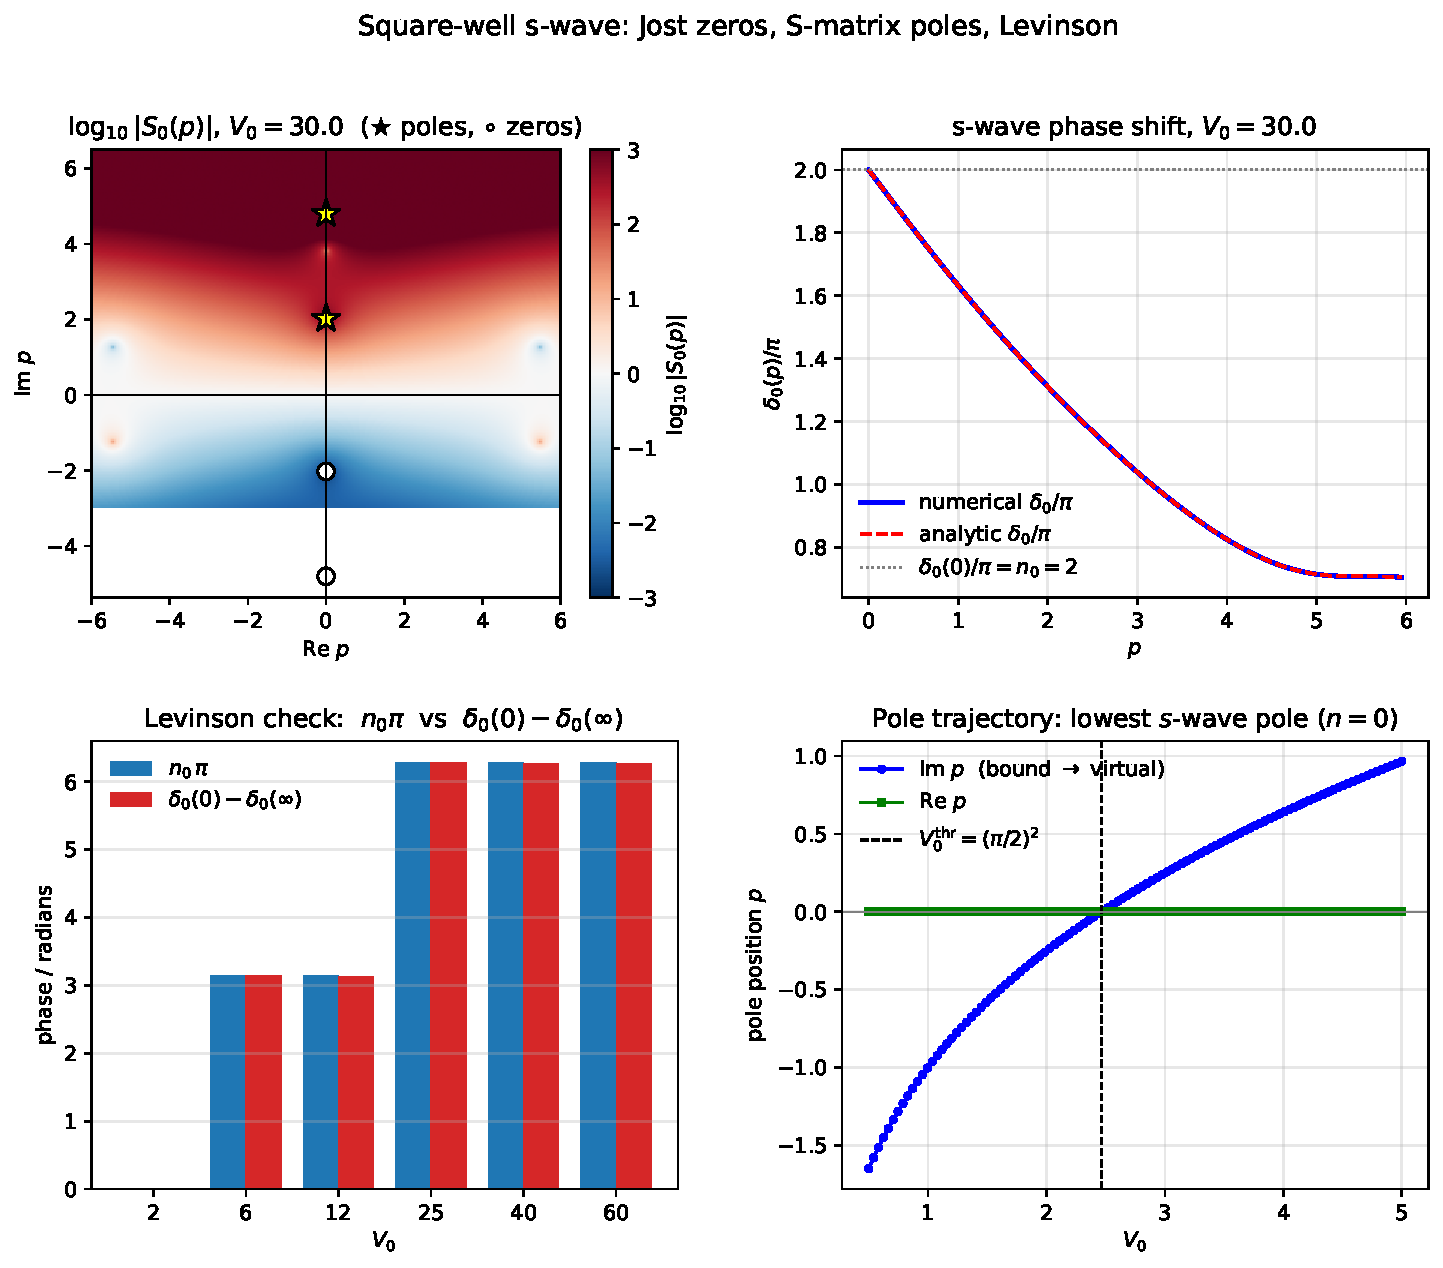
\includegraphics[width=0.95\linewidth]{ch11_jost_pole_levinson}
    \caption{方势阱 ($\hbar=2m=1,a=1$) s 波数值实验。
    \textbf{(左上)} $V_0=30$ 时复 $p$ 平面上 $\log_{10}|S_0(p)|$ 热图：
    黄色五角星标记上半平面 Jost 零点 $p=\rmi\kappa_{0,1}\approx\rmi\,2.022,\rmi\,4.800$ (S 矩阵极点)，
    白色圆点标记下半平面对应零点 ($S_0$ 的零点 $=\mathcal{F}_0(-p)$ 的零点)。
    \textbf{(右上)} 数值与解析相移对比：从 $\delta_0(0)/\pi=n_0=2$ 单调下降至 $0$，
    完全符合 Levinson 定理。
    \textbf{(左下)} 对一系列 $V_0$ 比较 $n_0\pi$ (束缚态计数) 与
    $\delta_0(0)-\delta_0(\infty)$ (相移积分)：两者数值上相等，相对误差 $<10^{-3}$。
    \textbf{(右下)} 当 $V_0$ 从 $5.0$ 降至 $0.5$ 时，最低 s 波 Jost 零点
    $p$ 沿虚轴向下穿过 $V_0^{\rm thr}=(\pi/2)^2\approx 2.467$ 时连续地由束缚态 $(\Im p>0)$
    转化为虚态 $(\Im p<0)$，$\Re p$ 始终为零 (s 波势阱中无共振分支)。}
    \label{fig:numexp-ch11}
\end{figure}

\subsection*{物理讨论}

\begin{enumerate}
\item \textbf{Jost 零点 $\leftrightarrow$ S 极点}：
由 $S_0(p)=\mathcal{F}_0(-p)/\mathcal{F}_0(p)$，$\mathcal{F}_0$ 的零点同时是 $S_0$ 的极点；
而 $\mathcal{F}_0(-p)$ 的零点是 $S_0$ 的零点。
解析延拓上 $\mathcal{F}_0(-p)=\overline{\mathcal{F}_0(\bar p)}$ (实势 Schwartz 反射)，
故上半平面的极点与下半平面的零点呈共轭分布
——这正是图 \ref{fig:numexp-ch11} 左上面板所展示的对称结构。

\item \textbf{束缚态、虚态、共振的统一刻画}：
    \begin{itemize}
    \item \emph{束缚态}: $p=\rmi\kappa$, $\kappa>0$, 即上半虚轴。能量 $E=-\kappa^2<0$ 物理上对应可归一束缚态。
    \item \emph{虚态}: $p=-\rmi\kappa$, $\kappa>0$, 即下半虚轴。同样对应实负能量但波函数发散，
          属第二叶。当势阱过浅以致最低束缚态消失时，对应的极点滑过 $p=0$ 进入下半轴成为虚态
          (右下面板)。两侧轨迹切线方向为 $\Im p\propto\pm\sqrt{|V_0-V_0^{\rm thr}|}$，对应阈
          能量行为 $E\propto V_0-V_0^{\rm thr}$。
    \item \emph{共振}: 第二叶上 $p_R=p_R'-\rmi p_R''$, $p_R'',p_R'>0$。s 波单纯方势阱不产生共振
          (无离心壁垒)，故图中未出现脱离虚轴的极点。共振在高分波或排斥壳中出现，将在
          \S\ref{ch:resonance} 集中讨论。
    \end{itemize}

\item \textbf{Levinson 定理 $\delta_0(0)-\delta_0(\infty)=n_0\pi$}：
左下面板把束缚态计数 $n_0$ (整数离散信息) 与连续相移 $\delta_0(p)$ 在物理域上的渐近差
(连续解析信息) 等同起来。
从全平面图像看，这是辐角原理 (argument principle)：
$\frac{1}{2\pi\rmi}\oint_C \frac{\mathcal{F}_0'(p)}{\mathcal{F}_0(p)}\,\rmd p=\#\text{零点}$，
取 $C$ 为上半平面无穷大半圆即得 Levinson；
该公式把分散在物理散射数据中的"积分相位"与上半平面"束缚态点谱"严格联系。
本数值实验取 $p_{\max}=2000$ 即足以让相移收敛到 $\delta_0(\infty)\bmod\pi=0$，
从而 $n_0\pi$ 与 $\delta_0(0)-\delta_0(\infty)$ 在 $\sim10^{-3}\pi$ 精度内吻合。

\item \textbf{阈值行为与零能反常}：
当 $V_0=V_0^{\rm thr}$ 时 $\mathcal{F}_0(0)=0$，即 S 矩阵在 $p=0$ 出现一阶极点，
散射长度 $a_s=-\lim_{p\to 0}\delta_0/p\to\infty$ (Wigner 散射阈值反常)。
右下面板的轨迹在 $V_0^{\rm thr}$ 处穿越原点，正是这一散射长度发散的直接图像。
冷原子物理中 Feshbach 共振调控正是利用了这种"束缚态—虚态"穿越机制。

\item \textbf{与全章解析结构的对应}：
方势阱不存在 Yukawa 型左割线 (势是紧支撑的)，故 $\mathcal{F}_0(p)$ 是整函数，
解析结构最为简洁——只有上下虚轴上的零点和左/右半平面的共振 (本例无)。
这恰好对应 \S\ref{ch:Smat1P} 提到的"截断势 $\Rightarrow$ Jost 函数解析至全平面"
的特殊情形，是检验本章一般理论的最干净的实验台。
\end{enumerate}
